\documentclass{beamer}
\usepackage[utf8]{inputenc}
\usepackage{paralist}
\usepackage[ngerman]{babel}
\usepackage{amsmath}
\usepackage{graphicx}
\usepackage{xcolor}
\usepackage{pdflscape}
\usepackage{color}
\usepackage{colortbl}
\usepackage{tabularx}
\usepackage{multirow}
\usepackage{algorithm}
\usepackage{algcompatible}
\usepackage{algorithmicx}
\usepackage{algpseudocode}
\usepackage{hyperref}
%\usepackage{utopia} %font utopia imported
%packages of house work
\usepackage{tabularray}
\usepackage{diagbox}
\usepackage{tikz}
\usetikzlibrary{shapes} 
\usepackage{pgfplots}
\usepackage{pgfplotstable}
\usepackage{tikz}
\usetikzlibrary{arrows.meta}
\usepackage{filecontents}
\usepackage[utf8]{inputenc}
\usepackage[ngerman]{babel}
%\usepackage[american]{babel}
\setcounter{secnumdepth}{4}
\usepackage{pdflscape}
\usepackage{lipsum}
\usepackage{mdwlist}
\usepackage{graphicx}
\usepackage{tabularx}
\usepackage{multirow}
\usepackage{rotating}
\usepackage{color}
\usepackage{colortbl}
\usepackage{multicol}
\usepackage{amsmath}
\usepackage{amsthm}
\usepackage{amssymb}
\usepackage{algorithm}
\usepackage{algcompatible}
\usepackage{algorithmicx}
\usepackage{algpseudocode}
\algblock[Class]{Class}{End}
\usepackage{wrapfig}
\usepackage{float}
\usepackage{url}
\usepackage{pdfpages}
\usepackage{cprotect}
\usepackage{setspace}
\usepackage{nomencl}
\usepackage{listings} 
\usepackage{cleveref}
\usepackage{rotating}
\usepackage{tikz}
\usepackage{adjustbox}
\usepackage{lscape}
\algrenewcommand\algorithmicrequire{\textbf{Input}}
\algrenewcommand\algorithmicensure{\textbf{Output}}
\renewcommand\algorithmiccomment[1]{\hfill$\triangleright\,$\textit{#1}}
\newcommand{\RNum}[1]{\uppercase\expandafter{\romannumeral #1\relax}}
\algrenewtext{Function}[2]{\algorithmicfunction\ \texttt{#1(#2)}}
\algnewcommand\algorithmicforeach{\textbf{for each}}
\algdef{S}[FOR]{ForEach}[1]{\algorithmicforeach\ #1\ \algorithmicdo}

\lstset{language=Python}
\lstset{frame=lines}
%\lstset{caption={Insert code directly in your document}}
%\lstset{label={lst:code_direct}}
%\lstset{basicstyle=\footnotesize}
\usepackage{xcolor}

\definecolor{codegreen}{rgb}{0,0.6,0}
\definecolor{codegray}{rgb}{0.5,0.5,0.5}
\definecolor{codepurple}{rgb}{0.58,0,0.82}
\definecolor{backcolour}{rgb}{0.95,0.95,0.92}

\usetheme{Madrid}
\usecolortheme{seahorse}

%------------------------------------------------------------
%This block of code defines the information to appear in the
%Title page
\title[Bachelorarbeit] %optional
{Das Wortproblem für kontextfreie Sprachen in subkubischer Zeit}

%\subtitle{Theorem von Simon}

\author[] % (optional)
{Ahmad Yassin}

\institute[] % (optional)
{
	Bachelorarbeit\\
}

\date\today

\AtBeginSection[]
{
	\begin{frame}<beamer>[noframenumbering]{Gliederung}
		\tableofcontents[currentsection]
	\end{frame}
}

\setbeamertemplate{bibliography item}{\insertbiblabel}


\begin{document}
	
	%The next statement creates the title page.
	\frame{\titlepage}
	\begin{frame}{Gliederung}
		\tableofcontents
	\end{frame}
	
	
	%---------------------------------------------------------
	
	
	\section{Einleitung}
	
	%---------------------------------------------------------
	%  Slide 1: Motivation 
	%---------------------------------------------------------

	\begin{frame}{Einleitung}
		\begin{block}{Wortproblem}
			Gegeben: Eine Grammatik $G = (S, \Sigma, N, P)$ und ein Wort $w$. \\
			Frage: Ist $w \in L(G)$? Dabei beschreibt $L(G)$ die Sprache, die durch $G$ erzeugt wird.
		\end{block}
		\pause
		\begin{itemize}
			\item Der Cocke-Younger-Kasami-Algorithmus (CYK) ist ein effizienter Algorithmus zur Lösung des Wortproblems für kontextfreie Sprachen.
			\item Die Zeitkomplexität des CYK-Algorithmus beträgt $O(n^{3})$.
			\item Gibt es Algorithmen mit besserer Zeitkomplexität als der CYK-Algorithmus?
			\pause
			\item Ja, es gibt viele, aber in dieser Arbeit werden wir uns den Leslie-G.-Valiant-Algorithmus (LGV) anschauen, der eine Zeitkomplexität von $O(n^{2.81})$ hat.
		\end{itemize}
	\end{frame}

	\begin{frame}{Ziel der Arbeit}
		\begin{itemize}
			\item Der LGV-Algorithmus hat bessere Laufzeiten als der CYK-Algorithmus.
			\pause
			\item Dazu werden beide Algorithmen implementiert.
			\pause
			\item Umwandlung in Chomsky-Normalform.
			\pause
			\item Die Implementierung erfolgt in Python Version 3.10.
			\pause
			\item Einsetzung dem Uni-Cluster, um die Laufzeiten zu messen.
		\end{itemize}
	\end{frame}
	
	%---------------------------------------------------------
	\section{Chomsky-Normalform}
	
		\begin{frame}{Chomsky-Normalform}
			\begin{definition}[\textbf{Chomsky-Normalform}]
				Eine kontextfreie Grammatik $G = (S, \Sigma, N, P)$ liegt in Chomsky-Normalform vor, wenn ihre Produktionen in einer von zwei einfachen Formen vorliegen:
				\begin{enumerate}
					\item $A \to BC$
					\item $A \to a$
				\end{enumerate}
			\end{definition}
			\pause
			Die Umwandlung in Chomsky-Normalform erfolgt in 4 Schritten:
			\begin{itemize}
				\item Eliminierung nutzloser Zeichen,
				\item Eliminierung von $\varepsilon$-Produktionen,
				\item Eliminierung von Einheitsproduktionen,
				\item Umwandlung in Chomsky-Normalform.
			\end{itemize}
		\end{frame}
		
		\begin{frame}{Eliminierung von nutzlosen Zeichen}
			Ein Zeichen $X$ in einer Grammatik $G = (S, \Sigma, N, P)$ wird als nutzlos bezeichnet, wenn es keine Ableitung der Form $S \to^{*} \alpha X \beta \to^{*} w$ gibt.
			\pause
			Diese Zeichen werden in zwei Gruppen unterteilt:
			\begin{enumerate}
				\item Die Gruppe der nicht-erzeugenden Zeichen besteht aus nichtterminalen Zeichen, die keine Kette von terminalen Zeichen erzeugen können.
				\item Die Gruppe der unerreichbaren Zeichen besteht aus terminalen und nichtterminalen Zeichen, die in keiner Ableitung von dem Startsymbol erreicht werden können.
			\end{enumerate}
			\pause
			Die Eliminierung der nutzlosen Zeichen erfolgt in zwei Schritten:
			\begin{enumerate}
				\item Suche nach nicht-erzeugenden Zeichen, um sie zu entfernen.
				\item Suche nach unerreichbaren Zeichen, um sie zu entfernen.
			\end{enumerate}
		\end{frame}
	
		\begin{frame}{Eliminierung von $\varepsilon$-Produktionen}
			Eine $\varepsilon$-Produktion ist eine Produktion der Form $A \to \varepsilon$ oder $A \to ^{*} \varepsilon$.
			\pause
			
			Die Eliminierung erfolgt in zwei Schritten:
			\begin{enumerate}
				\item Suche nach eliminierbaren nichtterminalen Zeichen und fasse sie in einer Menge zusammen.
				\item Entferne alle Produktionen, die auf Basis der erstellten Menge im vorherigen Schritt eliminiert werden können.
			\end{enumerate}
			
			\pause
			
			\begin{block}{Beispiel}
				Betrachte die Grammatik:
				$$(S, \{ a, b, c \}, \{ S, X \}, \{ S \to \ aSc | Sc | X, X \to aXb | Xb | \varepsilon \} )$$
				
				Nach der Eliminierung der $\varepsilon$-Produktionen ergibt sich:
				$$(S, \{ a, b, c \}, \{ S\}, \{ S \to aSc | Sc | X | ac |  c, X \to aXb | Xb | ab | b \})$$
			\end{block}
		\end{frame}
				
		\begin{frame}{Eliminierung von Einheitsproduktionen}
			Eine Einheitsproduktion ist eine Produktion der Form $A \to B$, wobei $A$ und $B$ nichtterminale Zeichen sind.
			\pause
			
			\begin{itemize}
				\item Einheitsproduktionen der Form $A \to B$ können nicht entfernt werden.
				\item Sie werden durch die Ersetzung von $B$ in der Produktion $A \to \alpha_1|\alpha_2|\ldots|\alpha_n$ behandelt.
				\item Dabei wird $B \to \alpha_1|\alpha_2|\ldots|\alpha_n$ verwendet.
			\end{itemize}
			
			\pause
			
			\begin{block}{Beispiel}
				Betrachte die Grammatik:
				$$(S, \{ a, b, c \}, \{ S\}, \{ S \to aSc | Sc | X | ac |  c, X \to aXb | Xb | ab | b \})$$
				
				Nach der Eliminierung der Einheitsproduktionen ergibt sich:
				$$(S, \{ a, b, c \}, \{ S\}, \{ S \to aSc | Sc | ac |  c | aXb | Xb | ab | b, X \to aXb | Xb | ab | b \})$$
			\end{block}
		\end{frame}
	
		\begin{frame}{Umwandlung in Chomsky-Normalform}
			Grammatiken, die durch die vorherigen Schritte bearbeitet wurden, besitzen weder nutzlose Zeichen noch $\varepsilon$-Produktionen noch Einheitsproduktionen.\\
			\pause
			Solche Grammatiken enthalten zwei verschiedene Arten von Produktionen:
			\begin{itemize}
				\item $A \to a$ - diese Produktion gilt als Chomsky-Normalform Produktion.
				\item $A \to \alpha_1, \alpha_2, \ldots ,\alpha_n$, wobei $\alpha_i \in \Sigma \cup N$ und $n \leq 2$ ist.
				\pause
				\begin{itemize}
					\item Ersetze alle $\alpha_i \in \Sigma$ durch $N_{\alpha_i} \to \alpha_i$ mit $N_{\alpha_i} \in N$.
					\item Ersetze $A \to \alpha_1, \alpha_2, \ldots ,\alpha_n$ durch $A \to \alpha_1 X_{\alpha_2}$, $X_{\alpha_2} \to \alpha_2 X_{\alpha_3}$, ..., $X_{\alpha_{n-1}} \to \alpha_{n-1} \alpha_n$ mit $X_{\alpha_i} \in N$.
				\end{itemize}
			\end{itemize}
			
			\pause
			
			\begin{block}{Beispiel}
				Betrachte die Grammatik:\\
				$(S, \{ a, b, c \}, \{ S\}, \{ S \to aSc | Sc | X | ac |  c | aXb | Xb | ab | b, X \to aXb | Xb | ab | b \})$
				Nach der Umwandlung in Chomsky-Normalform:
				$(S, \{ a, b, c \}, \{ S\}, \{ S \to AC|X_1|X_2|AB|AX_2|AX_1|b|c, X \to XB|AB|AX_1|b, X_1 \to XB , X_2 \to SC, A \to A, B \to B,C \to C\})$  
				 
			\end{block}
		\end{frame}
		
	
	\section{Cocke-Younger-Kasami-Algorithmus (CYK)}
	
%	\begin{frame}{Funktionalität}
%		Seien gegeben eine Grammatik $G = (S, \Sigma, N, P)$ in Chomsky-Normalform und ein Wort $w = \alpha_1 \alpha_2 \ldots \alpha_i \ldots \alpha_j\ldots \alpha_n$. Dabei funktioniert der CYK-Algorithmus wie folgt:
%		\begin{itemize}
%			\item Bottom-up-Prinzip, d.h. er versucht, ausgehend vom Wort $w$, auf das Startsymbol $S$ zurückzurechnen.
%			\pause
%			\item Suche nach einem Teilstring im aktuellen Wort 
%			$$w = \alpha_1 \alpha_2 \ldots \alpha_i \ldots \alpha_j\ldots \alpha_n$$
%			\item Der Teilstring $\alpha_i \ldots \alpha_j$ wird abgeleitet von $X \to \alpha_i \ldots \alpha_j \in P$
%			\pause
%			\item Ersetze den Teilstring mit $X$ im Wort
%			$$w_{neu} = \alpha_1 \alpha_2 \ldots X \ldots \alpha_{n-(j-i)+1}$$
%		\end{itemize}
%	\end{frame}
%	
%	\begin{frame}{Funktionalität}
%		\begin{block}{Beispiel}
%			Betrachte die Sprache: $$L = \{ a^{i}b^{j}c^{k} \ | \ i \leqslant j+k \}$$
%			Die Grammatik für diese Sprache lautet:$$G = (S,\ \ \{ a, \ b, \ c \}, \ \{A,\ C,\ X,\ B,\ Y_1,\ Y_2,\ S\}, \ P )$$
%			$$P=\{S \to SC\ |\ AB\ |\ AY_1\ |\ c\ |\ AY_2\ |\ b\ |\ XB\ |\ AC,$$ 
%			$$Y_1 \to SC, $$ 
%			$$ Y_2\to XB, $$ 
%			$$ X\to AY_2\ |\ AB\ |\ XB\ |\ b,$$
%			$$ A\to a,\ C\to c,\ B\to b\}$$
%		\end{block}
%	\end{frame}
%
%	\begin{frame}[plain]
%		\begin{figure}[ht]
%			\begin{tikzpicture}[scale=0.75]
%				\begin{scope}[every node/.style={circle,thick,draw}]
%					\node (A) at (0,0) {$v_1$};
%					\node (B) at (3,0) {$v_2$};
%					\node (C) at (6,0) {$v_3$};
%					\node (D) at (9,0) {$v_4$};
%					\node (E) at (12,0) {$v_5$};
%					\node (F) at (15,0) {$v_6$};
%				\end{scope}
%				
%				\begin{scope}[>={Stealth[black]},
%					every node/.style={fill=white,circle},
%					every edge/.style={draw=red}]
%					\path [->] (A) edge node {a} (B);
%					\path [->] (B) edge node {a} (C);
%					\path [->] (C) edge node {b} (D);
%					\path [->] (D) edge node {b} (E);
%					\path [->] (E) edge node {c} (F);
%				\end{scope}
%			\end{tikzpicture}
%		\end{figure}
%	\end{frame}
%
%	\begin{frame}[plain]
%		\begin{figure}[H]
%			\begin{tikzpicture}[scale=0.75]
%				\begin{scope}[every node/.style={circle,thick,draw}]
%					\node (A) at (0,0) {$v_1$};
%					\node (B) at (3,0) {$v_2$};
%					\node (C) at (6,0) {$v_3$};
%					\node (D) at (9,0) {$v_4$};
%					\node (E) at (12,0) {$v_5$};
%					\node (F) at (15,0) {$v_6$};
%				\end{scope}
%				
%				\begin{scope}[>={Stealth[black]},
%					every node/.style={fill=white,circle},
%					every edge/.style={draw=red}]
%					\path [->] (A) edge node {a} (B);
%					\path [->] (B) edge node {a} (C);
%					\path [->] (C) edge node {b} (D);
%					\path [->] (D) edge node {b} (E);
%					\path [->] (E) edge node {c} (F);
%					
%					\path [->] (A) edge [bend right=80] node {$A$} (B);%a%
%					\path [->] (B) edge [bend right=80] node {$A$} (C);%a%
%					\path [->] (C) edge [bend right=80] node {$S,B,X$} (D);%b%
%					\path [->] (D) edge [bend right=80] node {$S,B,X$} (E);%b%
%					\path [->] (E) edge [bend right=80] node {$S,C$} (F);%c%
%					
%					
%					%			\path [->] (A) edge [bend right=70] node {$\emptyset$}(B);%aa%
%					%			\path [->] (D) edge [bend right=70] node {$Y_1,S$}(E);%bc%
%					%			\path [->] (B) edge [bend right=70] node {$S,X$}(C);%ab%
%					%			\path [->] (C) edge [bend right=70] node {$S,X,Y_2$}(D);%bb%
%				\end{scope}
%			\end{tikzpicture}
%		\end{figure}
%	\end{frame}
%
%	\begin{frame}[plain]
%		\begin{figure}[H]
%			\begin{tikzpicture}[scale=0.75]
%				\begin{scope}[every node/.style={circle,thick,draw}]
%					\node (A) at (0,0) {$v_1$};
%					\node (B) at (3,0) {$v_2$};
%					\node (C) at (6,0) {$v_3$};
%					\node (D) at (9,0) {$v_4$};
%					\node (E) at (12,0) {$v_5$};
%					\node (F) at (15,0) {$v_6$};
%				\end{scope}
%				
%				\begin{scope}[>={Stealth[black]},
%					every node/.style={fill=white,circle},
%					every edge/.style={draw=red}]
%					\path [->] (A) edge node {a} (B);
%					\path [->] (B) edge node {a} (C);
%					\path [->] (C) edge node {b} (D);
%					\path [->] (D) edge node {b} (E);
%					\path [->] (E) edge node {c} (F);
%					
%					\path [->] (A) edge [bend right=80] node {$A$} (B);%a%
%					\path [->] (B) edge [bend right=80] node {$A$} (C);%a%
%					\path [->] (C) edge [bend right=80] node {$S,B,X$} (D);%b%
%					\path [->] (D) edge [bend right=80] node {$S,B,X$} (E);%b%
%					\path [->] (E) edge [bend right=80] node {$S,C$} (F);%c%
%					
%					\path [->] (B) edge [bend right=90] node {$S,X$}(D);%abb%
%					\path [->] (B) edge [bend right=100] node {$S,X,Y_2$}(E);%abb%
%					
%				\end{scope}
%			\end{tikzpicture}
%		\end{figure}
%	\end{frame}
%
%	\begin{frame}[plain]
%		\begin{figure}[H]
%			\begin{tikzpicture}[scale=0.75]
%				\begin{scope}[every node/.style={circle,thick,draw}]
%					\node (A) at (0,0) {$v_1$};
%					\node (B) at (3,0) {$v_2$};
%					\node (C) at (6,0) {$v_3$};
%					\node (D) at (9,0) {$v_4$};
%					\node (E) at (12,0) {$v_5$};
%					\node (F) at (15,0) {$v_6$};
%				\end{scope}
%				
%				\begin{scope}[>={Stealth[black]},
%					every node/.style={fill=white,circle},
%					every edge/.style={draw=red}]
%					\path [->] (A) edge node {a} (B);
%					\path [->] (B) edge node {a} (C);
%					\path [->] (C) edge node {b} (D);
%					\path [->] (D) edge node {b} (E);
%					\path [->] (E) edge node {c} (F);
%					
%					\path [->] (A) edge [bend right=80] node {$A$} (B);%a%
%					\path [->] (B) edge [bend right=80] node {$A$} (C);%a%
%					\path [->] (C) edge [bend right=80] node {$S,B,X$} (D);%b%
%					\path [->] (D) edge [bend right=80] node {$S,B,X$} (E);%b%
%					\path [->] (E) edge [bend right=80] node {$S,C$} (F);%c%
%					
%					\path [->] (B) edge [bend right=90] node {$S,X$}(D);%abb%
%					\path [->] (B) edge [bend right=90] node {$S,X,Y_2$}(E);%abb%
%					\path [->] (A) edge [bend right=95] node {$S,X$}(E);%abb%
%					\path [->] (A) edge [bend right=100] node {$S$}(F);%aabbc%
%					
%				\end{scope}
%			\end{tikzpicture}
%		\end{figure}
%	\end{frame}
	
	\begin{frame}{CYK-Algorithmus in pseudocode}
		Der CYK-Algorithmus könnte in pseudocode wie folgt aussehen:	
		\begin{block}{CYK-Algorithmus}
			Eingabe: Grammatik $G = (S, \Sigma, N, P)$ in Chomsky-Normalform und ein Wort $w=a_1 \ldots a_n \in \Sigma^*$\\
			Ausgabe: $\mathrm{w} \in \mathrm{L}(\mathrm{G})$ (falls w von G erzeugt wird), sonst $\notin \mathrm{L}(\mathrm{G})$\\
			(i) for $\mathrm{i}:=1$ to $\mathrm{n}$ do\\
			\ \ \ \ \ \ \ \ \ \ $\mathrm{N}_{\mathrm{i}, \mathrm{i}}:=\left\{\mathrm{A} \in \mathrm{N} \mid \mathrm{A} \rightarrow \mathrm{a}_{\mathrm{i}} \in \mathrm{P}\right\}$\\
			(ii) for $h:=1$ to $\mathrm{n}-1$ do\\
			\ \ \ \ \ \ \ \ \ \ \ \ for $i:=1$ to $n-h$ do\\
			\ \ \ \ \ \ \ \ \ \ \ \ \ \ \ \ \ \ $\mathrm{N}_{\mathrm{i}, \mathrm{i}+\mathrm{h}}=\bigcup_{j=i}^{i+h-1} \mathrm{N}_{i, j} \cdot \mathrm{~N}_{j+1, i+h}$\\
			(iii) if $S \in \mathrm{N}_{1, \mathrm{n}}$\\
			\ \ \ \ \ \ \ \ \ \ then Ausgabe $\mathrm{w} \in \mathrm{L}(\mathrm{G})$\\
			\ \ \ \ \ else\\
			\ \ \ \ \ \ \ \ \ \  Ausgabe w $\notin \mathrm{L}(\mathrm{G})$
		\end{block}
	\end{frame}

	\begin{frame}{CYK-Algorithmus in pseudocode}
		Die Operation $\cdot$ ist wie folgt definiert:
		\begin{block}{\textbf{$N_1 \ \cdot \ N_2$}}
			Sei $G = (S, \Sigma, N, P)$ eine Grammatik in Chomsky-Normalform und seien $N_1,N_2 \subseteq N$, dann gilt:
			$$N_1 \ \cdot \ N_2 = \{A \ |\ \exists  B\in N_1 , \exists C\in N_2 : A\to BC \in P\}$$
		\end{block}
		\pause
		\begin{figure}[H]
			\begin{table}[H]
				\centering
				\begin{tabular}{|m{1cm}||m{1cm}|m{1cm}|m{1cm}|m{1cm}|m{1cm}|} 
					\hline
					& $\mathbf{w_1}$ & $\mathbf{w_2}$ & $\mathbf{w_3}$ & $\mathbf{w_4}$ & $\mathbf{w_5}$  \\
					\hline\hline
					$\mathbf{w_1}$ & \cellcolor{brown} $L_{[1,1]}$ &  \cellcolor{gray}$L_{[1,2]}$ &  \cellcolor{green} $L_{[1,3]}$&  \cellcolor{blue} $L_{[1,4]}$& \cellcolor{red} $L_{[1,5]}$ \\
					\hline
					$\mathbf{w_2}$ &  $L_{[2,1]}$& \cellcolor{brown} $L_{[2,2]}$ &  \cellcolor{gray} $L_{[2,3]}$&  \cellcolor{green} $L_{[2,4]}$& \cellcolor{blue} $L_{[2,4]}$\\
					\hline
					$\mathbf{w_3}$ &  $L_{[3,1]}$&  $L_{[3,2]}$& \cellcolor{brown} $L_{[3,3]}$&  \cellcolor{gray} $L_{[3,4]}$& \cellcolor{green} $L_{[3,5]}$\\
					\hline
					$\mathbf{w_4}$ &  $L_{[4,1]}$&  $L_{[4,2]}$&  $L_{[4,3]}$& \cellcolor{brown} $L_{[4,4]}$& \cellcolor{gray} $L_{[4,5]}$\\
					\hline
					$\mathbf{w_5}$ &  $L_{[5,1]}$&  $L_{[5,2]}$&  $L_{[5,3]}$&  $L_{[5,4]}$& \cellcolor{brown} $L_{[5,5]}$\\
					\hline
				\end{tabular}
			\end{table}
		\end{figure}
	\end{frame}

	\begin{frame}{Komplexitätzeit und Implementierung}
		\begin{algorithm}[H]
			\floatname{algorithm}{Algorithmus}
			\setstretch{1.1}
			\caption[Teil (i)]{Teil (i)}
			\label{algorithm9}
			\begin{algorithmic}[1]
				\For{\texttt{$i:=1 \ to \ n$}}  \ \ \ \ \ \ \ \ \ \ \ \ \ \ \ \ \ \ \ \ \ \ \ \ \ \ \ \ \ \ \ \ \ \ \ \ \ \ \ \ \ \ \textbf{$ \%O(n)$ Durchläufe}
				\ForEach { $A\to\alpha \in P$} \ \ \ \ \ \ \ \ \ \ \ \ \ \ \ \ \ \ \ \ \ \ \ \ \ \ \ \ \textbf{$\%O(|P|)$ Durchläufe}
				\If{$A\to\alpha = B \to w_i$}
				\State Füge $A$ zur Menge des Listenelements $L_{[i,i]}$
				\Else
				\State Abbruch (Das Wort $w$ ist nicht ableitbar)
				\EndIf
				\EndFor
				\EndFor
			\end{algorithmic}
		\end{algorithm}
	\end{frame}

	\begin{frame}{Komplexitätzeit und Implementierung}
		\begin{algorithm}[H]
			\floatname{algorithm}{Algorithmus}
			\setstretch{1.1}
			\caption[Teil (ii)]{Teil (ii)}
			\label{algorithm10}
			\begin{algorithmic}[1]
				\For{\texttt{$h:=1 \ to \ n$}} \ \ \ \ \ \ \ \ \ \ \ \ \ \ \ \ \ \ \ \ \ \ \ \ \ \ \ \ \ \ \ \ \ \ \ \ \ \ \ \ \ \ \textbf{$ \%O(n)$ Durchläufe}
				\For{\texttt{$i:=1 \ to \ n-h$}} \ \ \ \ \ \ \ \ \ \ \ \ \ \ \ \ \ \ \ \ \ \ \ \ \ \ \ \ \ \ \ \ \ \textbf{$ \%O(n)$ Durchläufe}
				\For{\texttt{$j:=i \ to \ i+h-1$}} \ \ \ \ \ \ \ \ \ \ \ \ \ \ \ \ \ \ \ \ \ \ \ \ \textbf{$ \%O(n)$ Durchläufe}
				\ForEach { $A\to\alpha \in P$} \ \ \ \ \ \ \ \ \ \ \ \ \ \ \ \ \ \ \ \ \textbf{$\%O(|P|)$ Durchläufe}
				\If{$|\alpha| = 2 \land  \alpha_1 \in L_{[i,j]} \land  \alpha_2 \in L_{[j+1,i+h]}$}
				\State Füge $A$ zur Menge des Listenelements $L_{[i,i+h]}$
				\EndIf
				\EndFor
				\EndFor
				\EndFor
				\EndFor
			\end{algorithmic}
		\end{algorithm}
		 \href{http://www.cip.ifi.lmu.de/~lindebar/}{CYK-Algorithmus Funktionalität durch graphische Effekte}.
	\end{frame}
	
	%---------------------------------------------------------
	
	
	\section{Leslie-G.-Valiant-Algorithmus (LGV)}

	\begin{frame}{Leslie-G.-Valiant-Algorithmus (LGV)}
		\begin{figure}
			\centering
			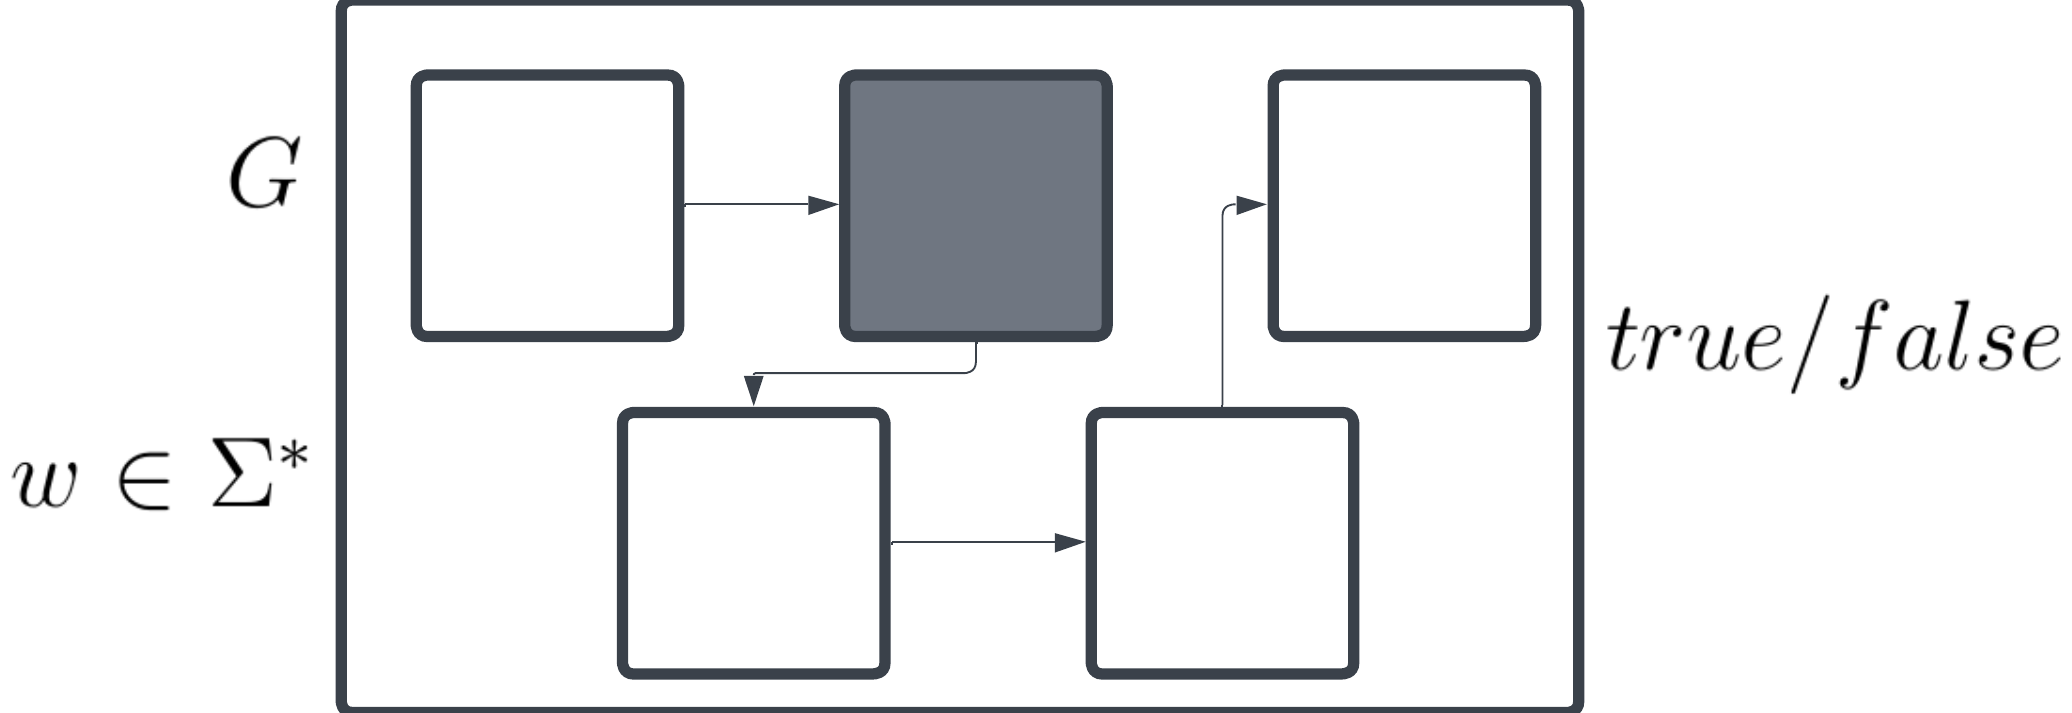
\includegraphics[width=11cm,height=4cm]{img/LGVT}
		\end{figure}
		\begin{itemize}
			\item Eingabe des LGV-Algorithmus:
			\begin{itemize}
				\item $G = (S, \Sigma, N, P)$ in Chomsky-Normalform.
				\item Wort der Länge $n=|w|$.
			\end{itemize}
			\pause
			\item Multiplikation von $n \times n$ booleschen Matrizen.
			\item Verwendung der Strassen-Matrix-Multiplikation.
			\item LGV-Algorithmus erreicht Zeitkomplexität von $O(n^{2.81})$.
			\pause
			\item Dies kann durch eine Reihe von Reduktionen gezeigt werden.
		\end{itemize}
	\end{frame}

	\begin{frame}{Leslie-G.-Valiant-Algorithmus (LGV)}
		\begin{figure}
			\centering
			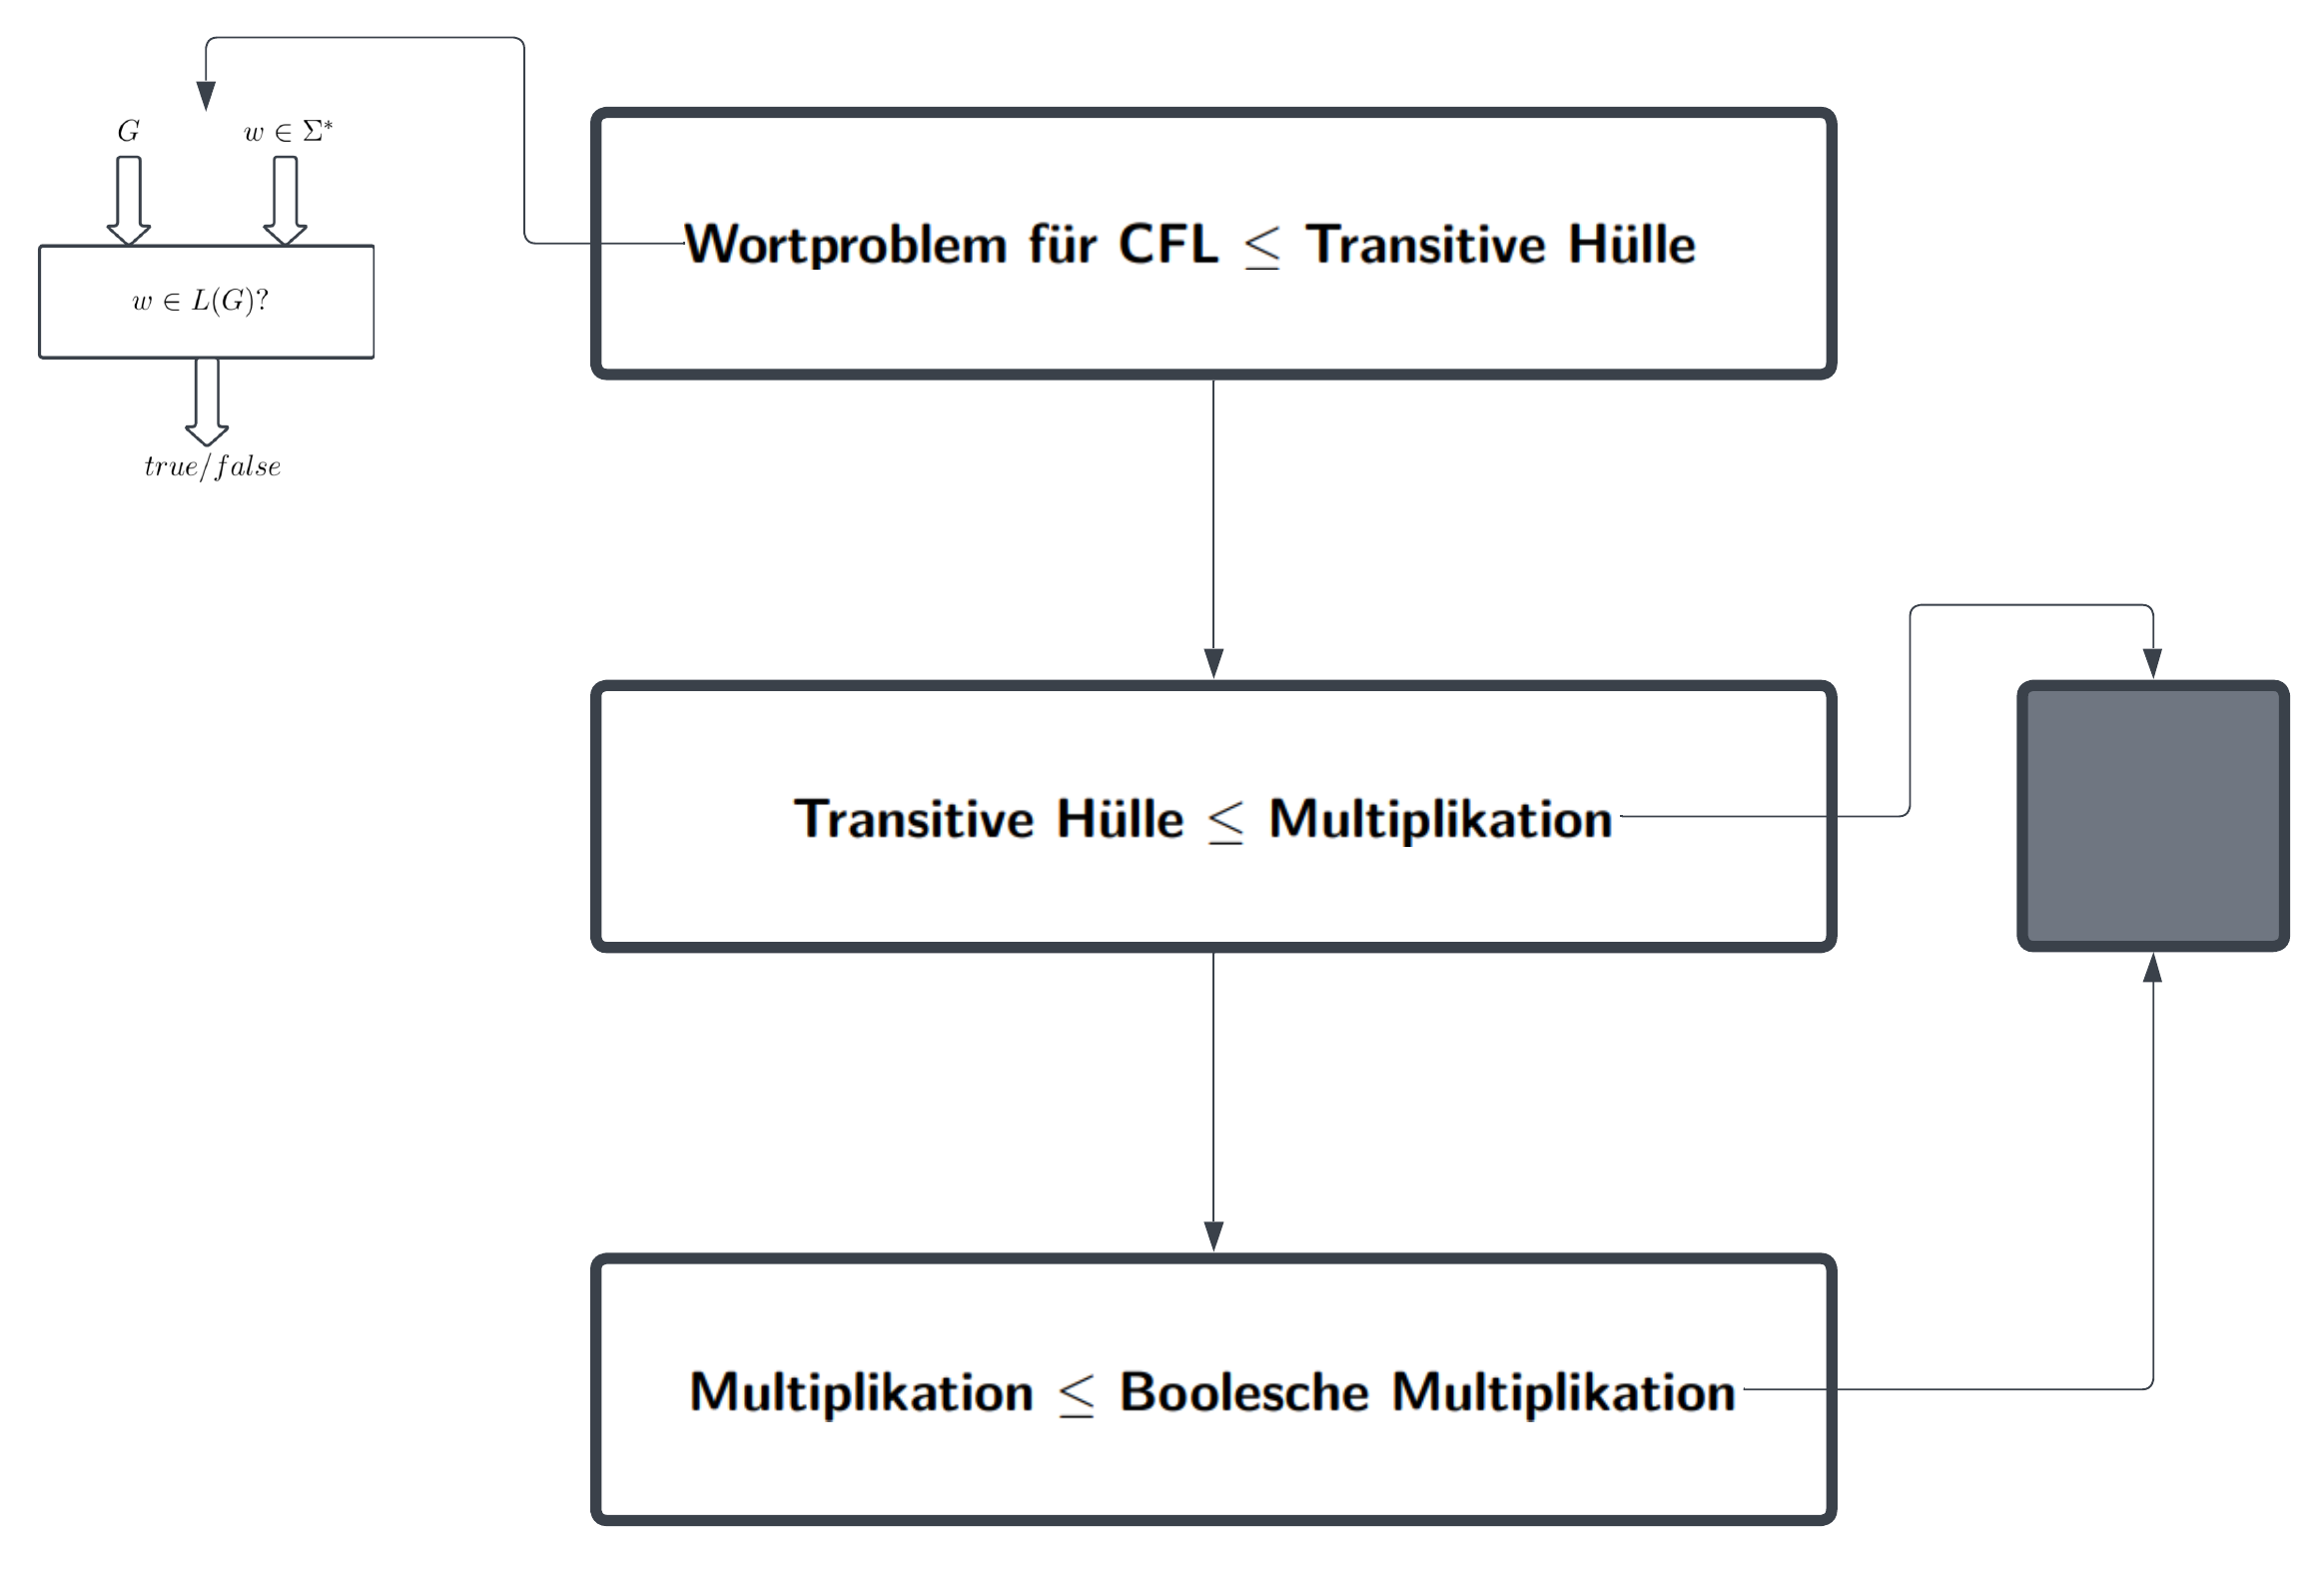
\includegraphics[width=10.5cm,height=7.5cm]{img/ZusammenfassungT}
		\end{figure}
	\end{frame}

	\begin{frame}{Preparation}
		\begin{itemize}
			\item Die Definition der Matrixmultiplikation lautet folglich $c = a \cdot b$
			$$\textcolor{blue}{c_{ik}} = \textcolor{green}{a_{i1}} \cdot \textcolor{red}{b_{1k}} \cup \ldots \cup \textcolor{green}{a_{in}} \cdot \textcolor{red}{b_{nk}} =  \bigcup_{j=1}^{n} a_{ij} \cdot b_{ik}$$
			\item Die transitive Hülle einer quadratischen Matrize a
			$$a^+ = a^{(1)} \cup a^{(2)} \cup \ldots$$
			\pause
			\item Dabei wird $a^{(i)}$ wie folgt definiert:
			$$a^{(i)} = \bigcup_{j=1}^{i-1} a^{(j)} \cdot a^{(i-j)} \  und \ a^{(1)} = a$$
			\item Die transitive Hülle für die Matrize $a$ ist endlich.
		\end{itemize}

	\end{frame}

	\begin{frame}{Preparation}
		\begin{itemize}
			\item Ein Hemiring $(H, \cup, \emptyset,\cdot)$
			\begin{itemize}
				\item $H$ ist die Potenzmenge von $N$,
				\item $\cup$ sowohl kommutativ als auch assoziativ,
				\item $\cdot$ weder kommutativ noch assoziativ,
				\item $\emptyset$ ist das Nullelement eines Hemirings, d. h.
				\begin{itemize}
					\item $\emptyset$ ist neutrales Element bezüglich dem Operator $\cup$
					\item $\emptyset$ ist absorbierend bezüglich dem Operator $\cdot$
				\end{itemize}
			\end{itemize}
			\pause
			\item Zeitkomplexitätsfunktionen
			\begin{itemize}
				\item $R(n)$ für das Lösen des Wortproblems.
				\item $M(n)$ für die Multiplikation von $n\times n$ Matrizen.
				\item $T(n)$ für das Finden der transitiven Hülle von $n  \times n$ oberen Dreiecksmatrizen.
				\item $BM(n)$ für das Multiplizieren von $n \times n$ booleschen Matrizen. 
			\end{itemize}
		\end{itemize}
	\end{frame}

	\begin{frame}{Wortproblem für CFL $\le$ Transitive Hülle}
		\begin{itemize}
			\item Sei $G = (S, \Sigma, N, P)$ eine Grammatik in Chomsky-Normalform und $w=w_1 w_2 \ldots w_n$ ein Wort über $\Sigma^*$.
			\pause
			\item Nun wird eine $(n+1)\times (n+1)$ obere Dreieckmatrix $b$ gebildet und wie folgt definiert:
			$$b_{i,i+1} = \{ A | A\to w_i \in P\} \ und \ b_{i,j}= \emptyset \ f\ddot{u}r \ alle \ j \neq i+1$$
			\pause
			\item Aus der Definition der Multiplikationsoperation ergibt sich induktiv, dass die
			Elemente der transitiven Hülle $b^+$ ausschließlich diejenigen sind, die die Eigenschaft haben, dass 
			$$A \in b_{i,j}^+ \Leftrightarrow A \to^* w_i \ldots w_{j-1}$$
			\pause
			\item Es kann also festgestellt werden, ob $S \to^* w$, indem $a = b^+$ berechnet und
			gefragt wird, ob $S \in a_{1,n+1}$ .
		\end{itemize}
	\end{frame}

	\begin{frame}{Wortproblem für CFL $\le$ Transitive Hülle}
		Korrektheit der Reduktion.
		\begin{itemize}
			\item Das Wort $w$ wird vom Startsymbol $S$ abgeleitet $\Longleftrightarrow$
			\item das Startsymbol $S$ in dem oberen rechten Eintrag $a_{1,n+1}$ der Matrize $b^+$ zu finden ist.
			\pause
			\item Unter Berücksichtigung des Aufwands für die Erstellung der oberen Dreieckmatrix $b$ entsteht die folgende Zeitkomplexität.
		\end{itemize}
		\begin{block}{Theorem}
			$R(n) \le T(n+1) + O(n^2)$
		\end{block}
	\end{frame}

	\begin{frame}{Transitive Hülle $\le$ Multiplikation}
		\begin{block}{Lemma}
			Sei $b$ eine obere Dreiecksmatrix der Größe $n \times n$. Unter der Annahme, dass die transitive Hülle der Partitionen $[1\le i,j\le r]$ und $[n-r < i,j\le n]$ für ein $r > \frac{n}{2}$ bekannt sind, kann der Abschluss von $b$ wie folgt berechnet werden:
			\begin{enumerate}
				\item Durchführung einer einzigen Matrixmultiplikation.
				\item Finden der transitiven Hülle einer oberen Dreiecksmatrix der Größe $2(n-r) \times 2(n-r)$, für die die Hülle der Partitionen $[1\le i,j\le n-r]$ und $[n-r < i,j\le 2(n-r)]$ bekannt sind.
			\end{enumerate}
		\end{block}
	\end{frame}

	\begin{frame}{Transitive Hülle $\le$ Multiplikation}
		\begin{figure}
			\centering
			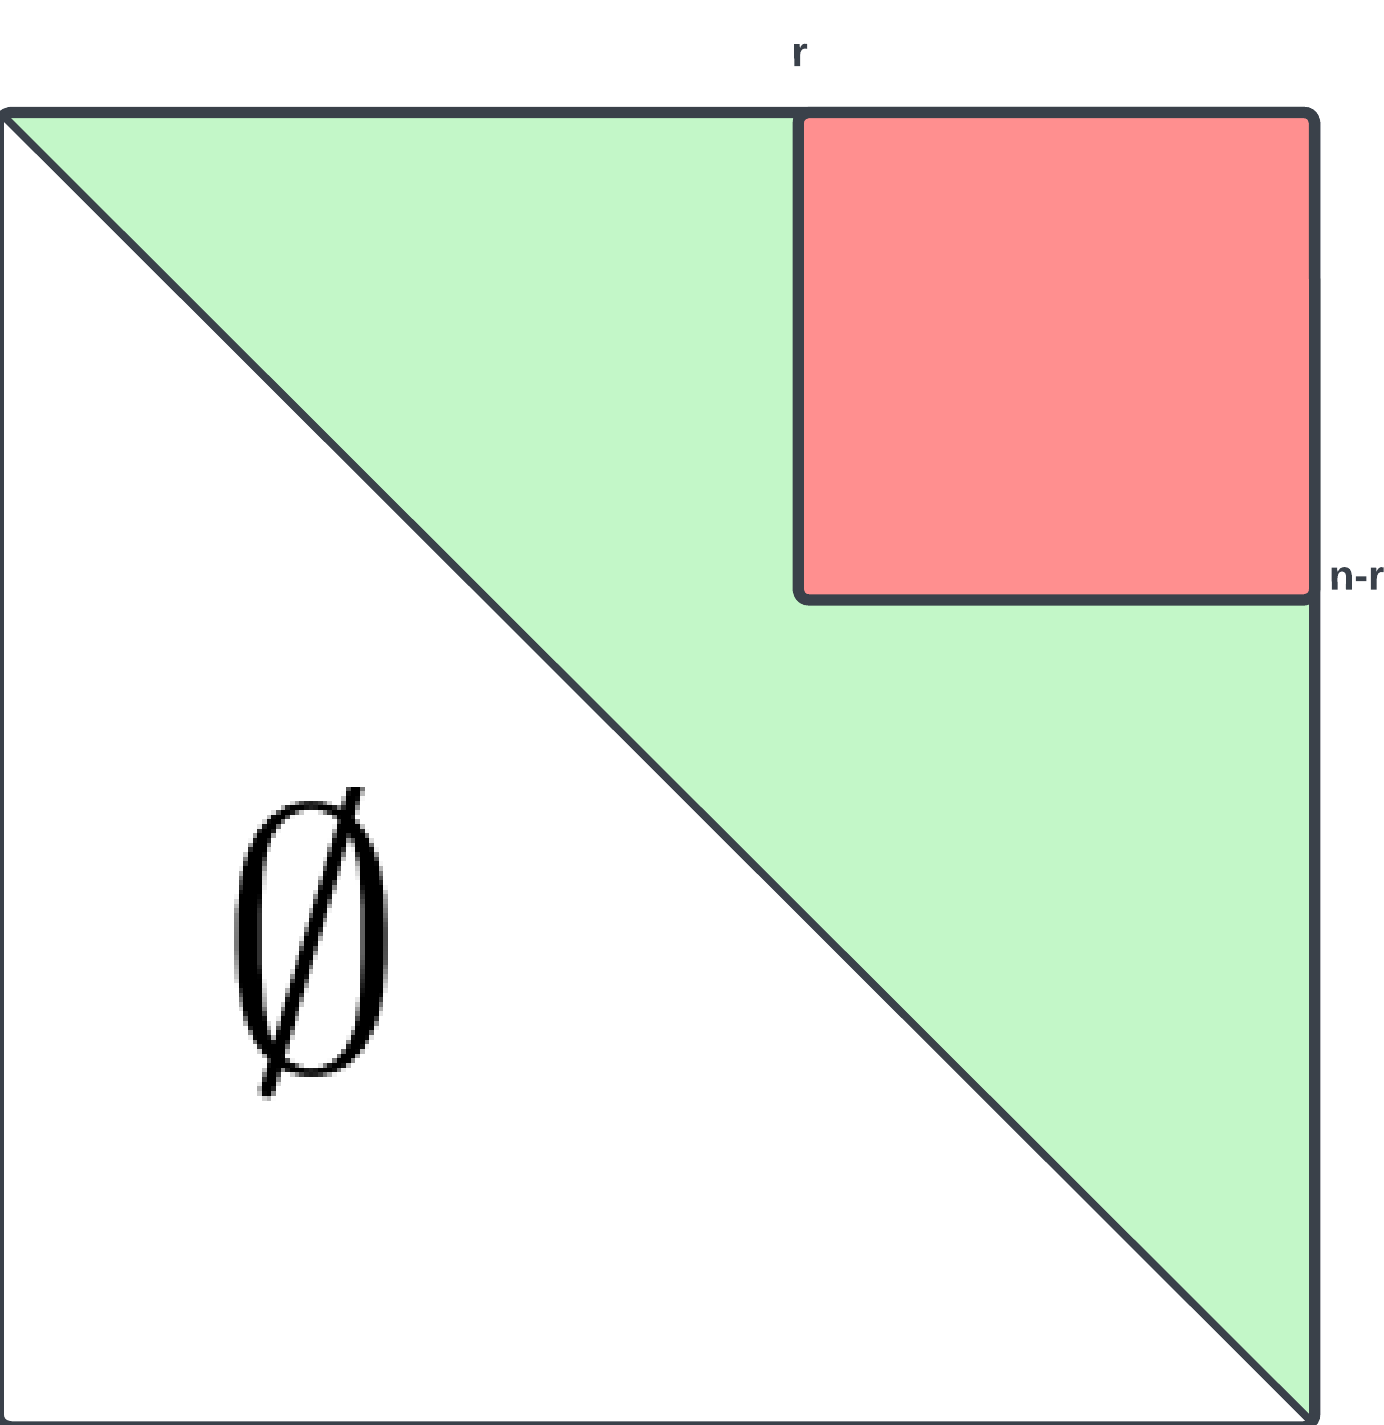
\includegraphics[width=7cm,height=7cm]{img/LGV1}
		\end{figure}
	\end{frame}

	\begin{frame}{Transitive Hülle $\le$ Multiplikation}
		\begin{itemize}
			\item Ein Term ist die Zusammensetzung von Matrixelementen unter $(\cdot)$
			\item Die binäre Operation $\cdot$ ist nicht assoziativ
			\item Terme können verschiedene Assoziationsordnungen haben
			\item $(2, 11)$-Terme
			\begin{itemize}
				\item $(b_{2,5}\cdot (b_{5,7}\cdot b_{7,8}))\cdot b_{8,11}$
				\item $(b_{2,5}\cdot (b_{5,7}\cdot (b_{7,8}\cdot b_{8,11})))$
			\end{itemize}
			\pause
			\item Induktiv könnte gezeigt werden, dass
			\begin{itemize}
				\item $b_{k,l}^{(i)}$ ist die Vereinigung aller formal verschiedenen $(k,l)$-Terme mit genau $i$ Komponenten
				\item $b_{k,l}^+$ ist gleich die Vereinigung aller formal verschiedenen $(k, 1)$-Terme
			\end{itemize}
			\item Lediglich die obere rechte Partition von $b^+$ muss berechnet werden
			 
		\end{itemize}
	\end{frame}
	
	\begin{frame}{Transitive Hülle $\le$ Multiplikation}
		\begin{itemize}
			\item In jedem $(k, l)$-Term gibt es einen minimalen $(p, q)$-Unterterm. 
			\item Jeder dieser minimalen Teilterme hat
			\begin{itemize}
				\item entweder nur eine Komponente, den $(p,q)$-Term
				\item oder ist die Zusammensetzung von $(p, s)$ $(s, q)$ Terme.
			\end{itemize}
			\pause
			\item Die Vereinigung aller möglichen formal verschiedenen minimalen $(p,q)$-Unterterme ist
			$$b_{pq} \cup \bigcup_{n-r < s \le r}^{} b_{ps}^+ \cdot b_{sq}^+$$
			\pause
			\item $b_{ps}^+$ und $ b_{sq}^+$ sind durch die Annahme bekannt
			$$c^{'} = b_{ps}^+ \cdot b_{sq}^+$$
			$$c = c^{'} \cup b_{pq}$$
			\item Matrix $c$ ist gleich der Vereinigung aller formal verschiedenen minimalen $(p, q)$-Terme von $b$ ist.
		\end{itemize}
	\end{frame}

	\begin{frame}{Transitive Hülle $\le$ Multiplikation}
		\begin{figure}
			\centering
			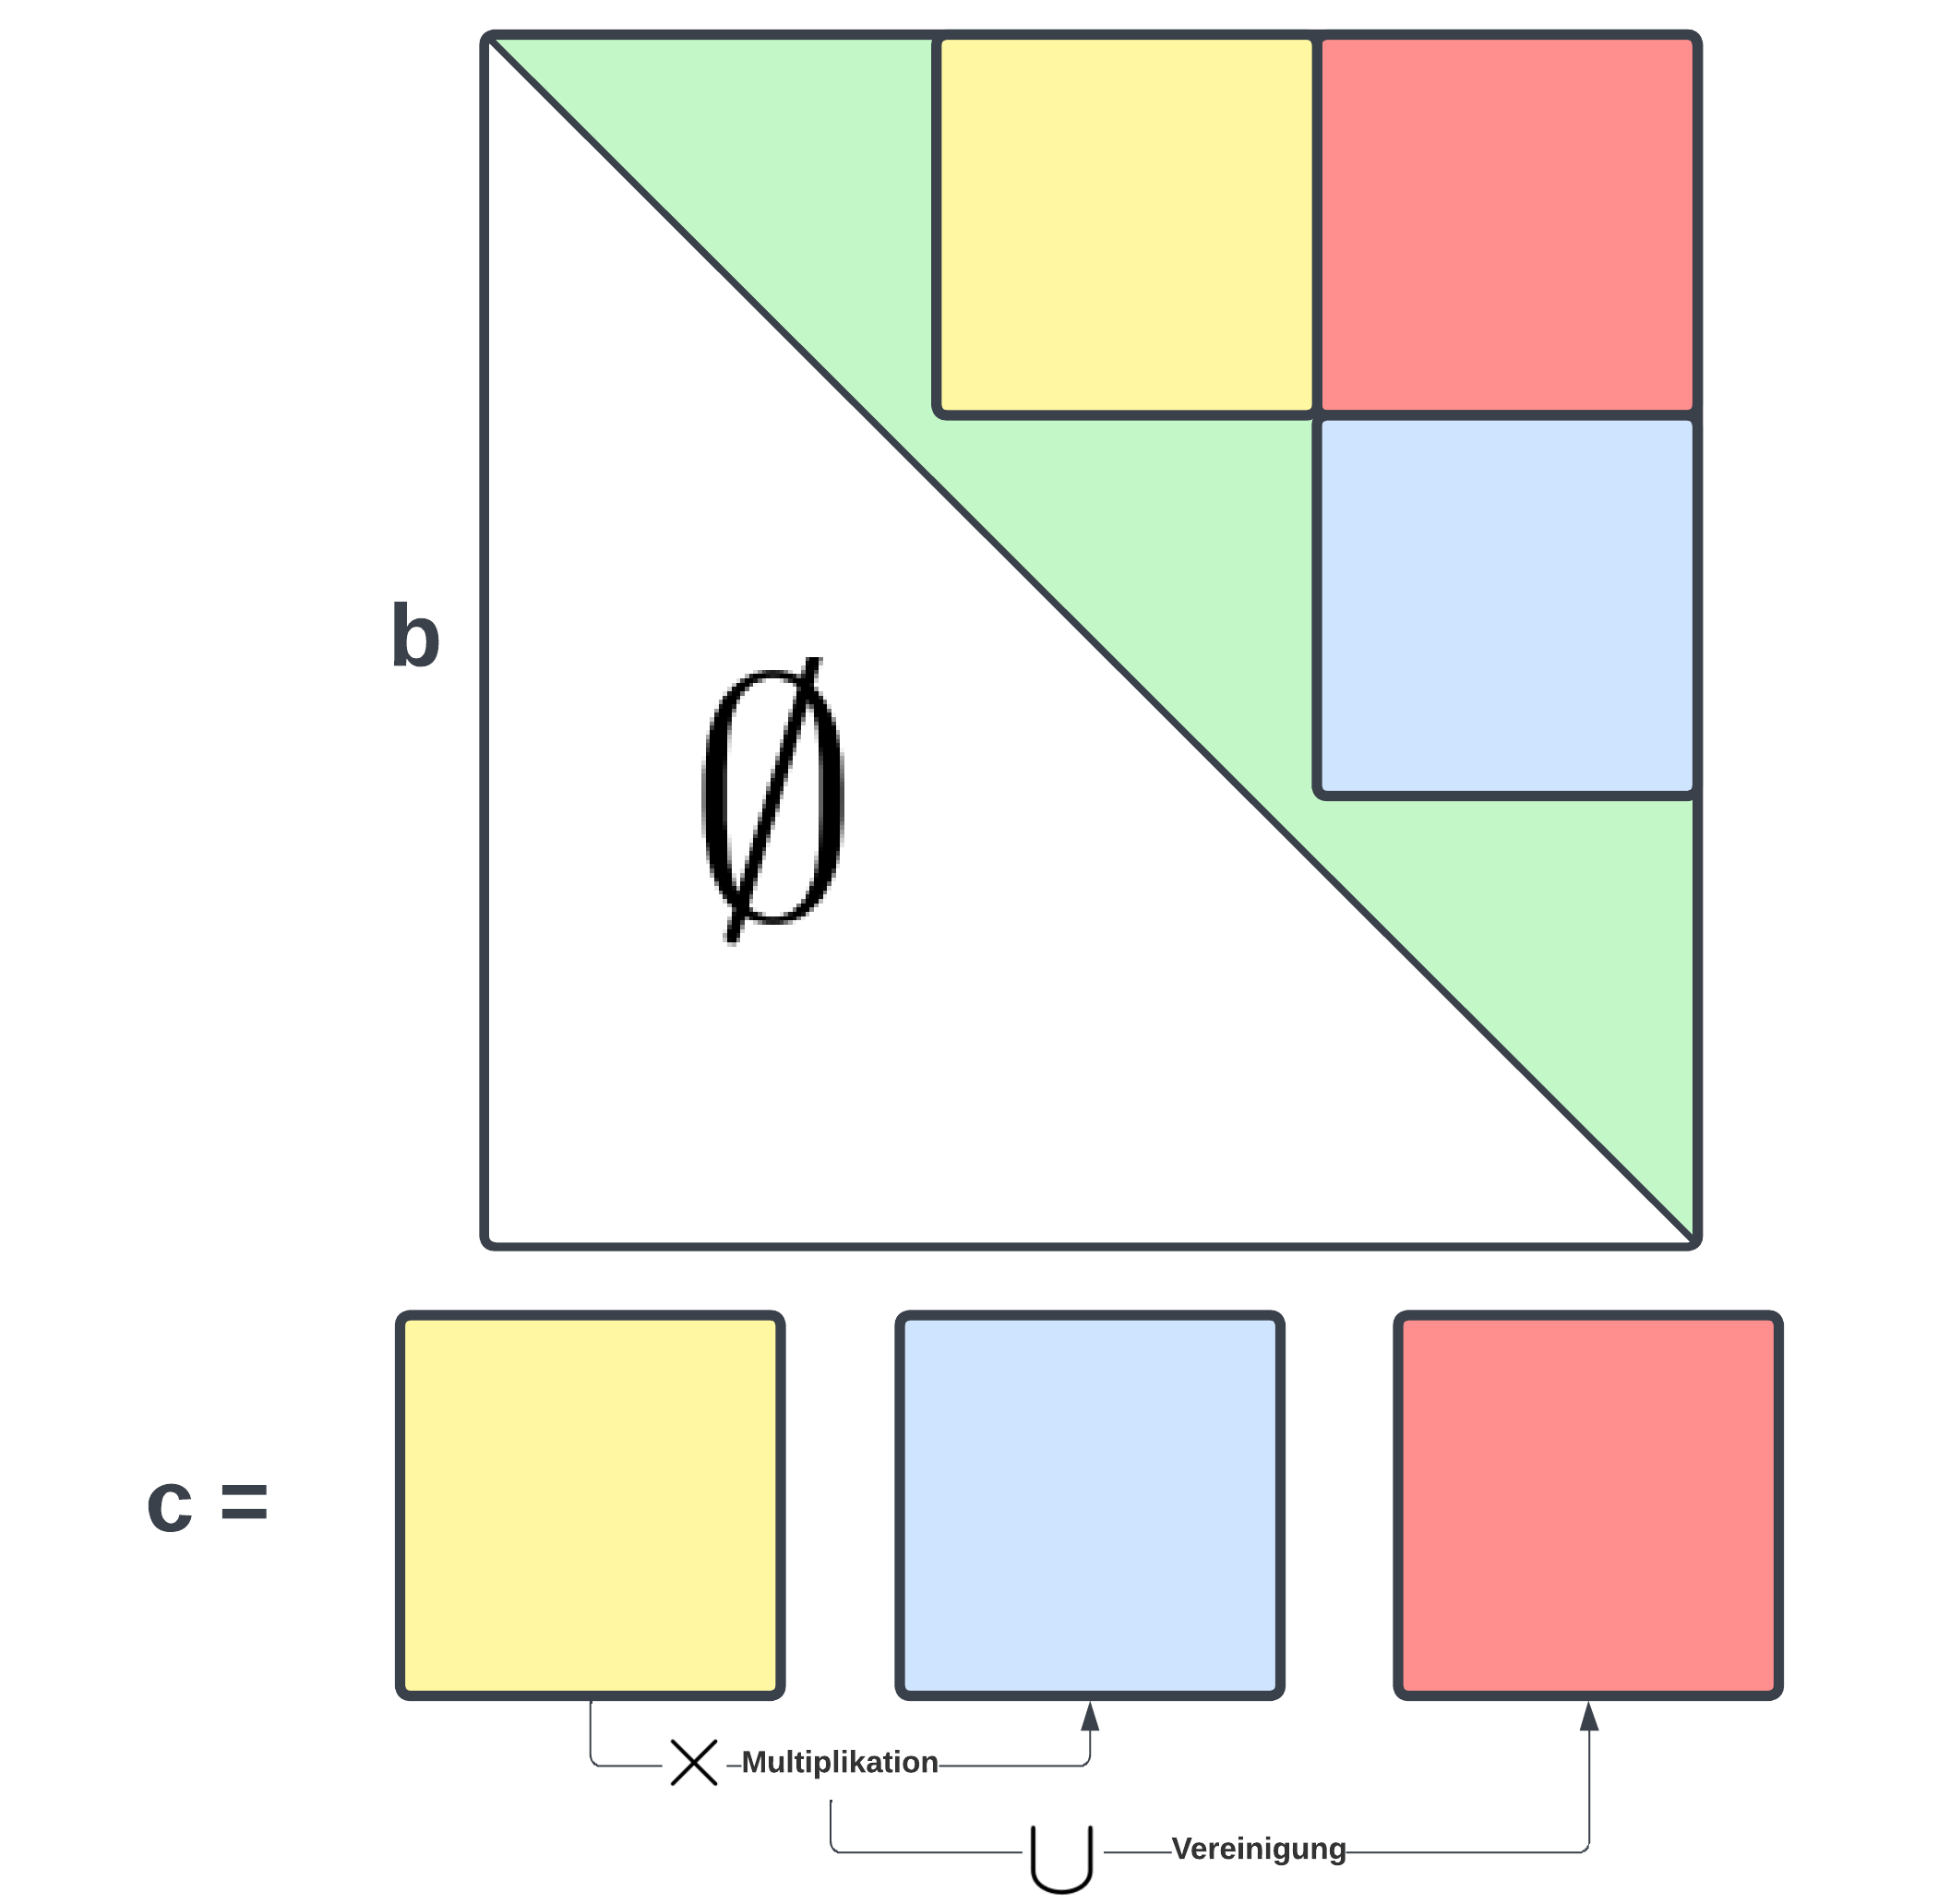
\includegraphics[width=7.5cm,height=7.5cm]{img/LGV2}
		\end{figure}
	\end{frame}

	\begin{frame}{Transitive Hülle $\le$ Multiplikation}
		\begin{figure}
			\centering
			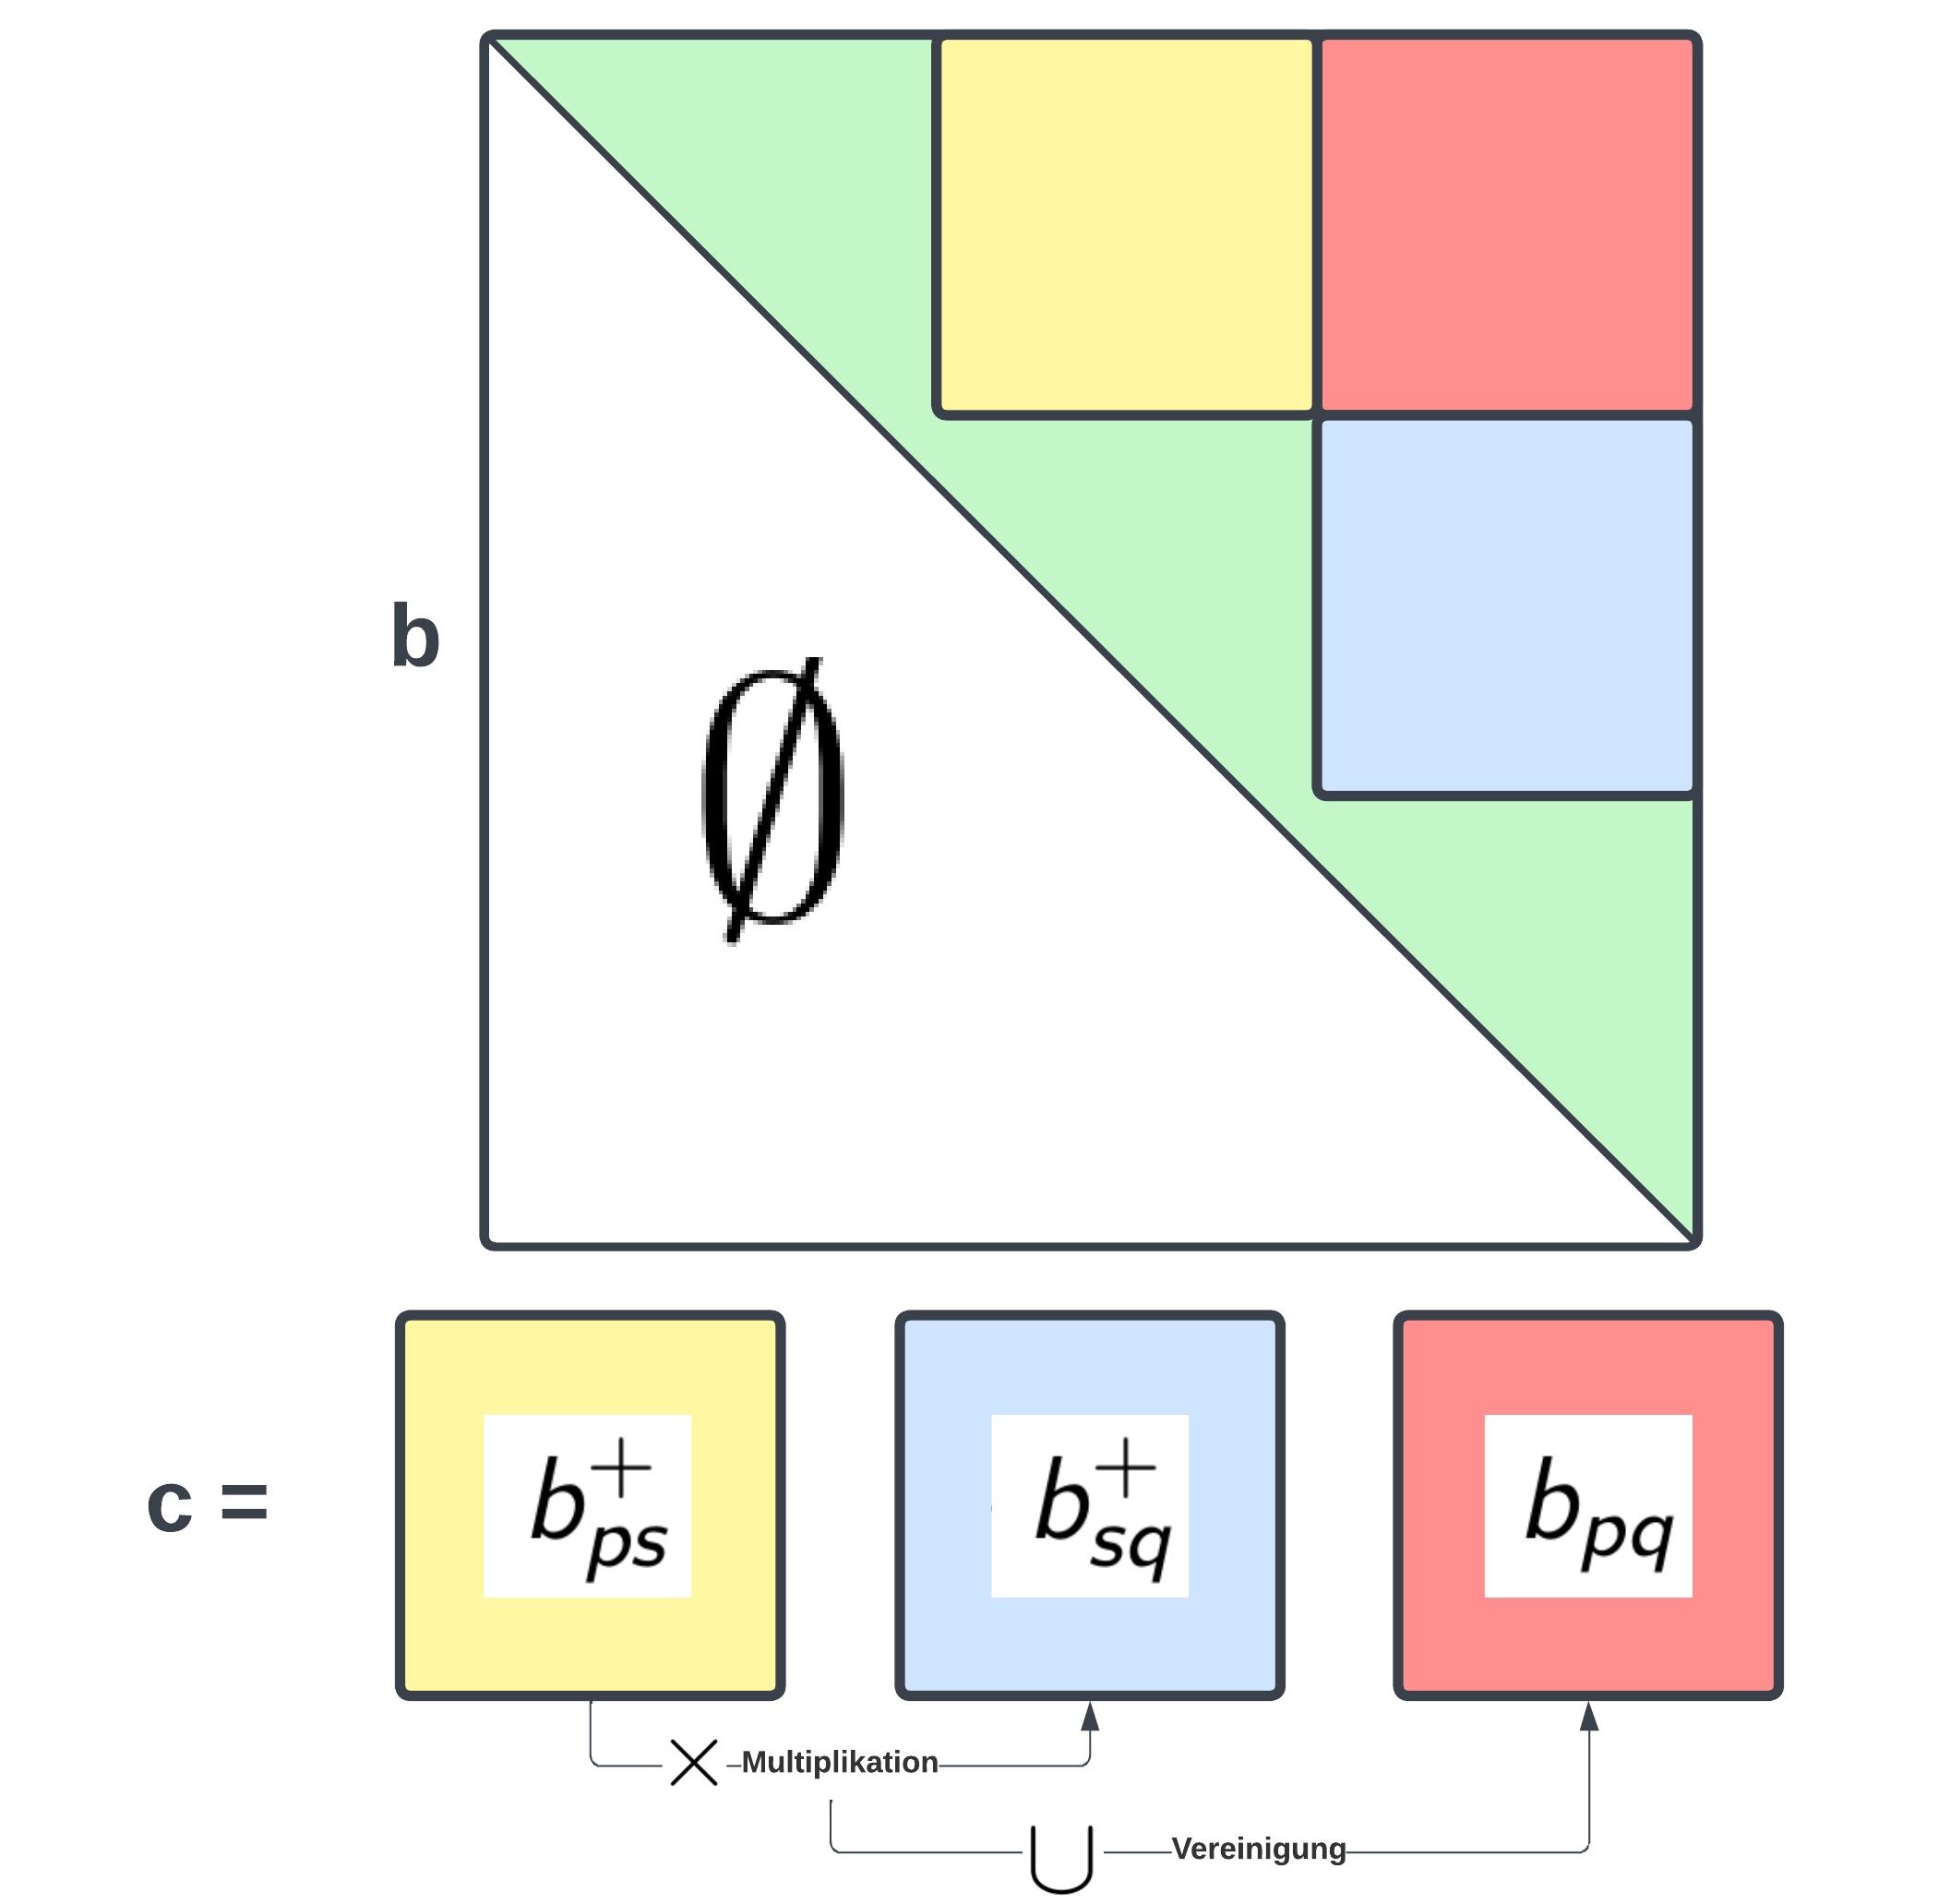
\includegraphics[width=7cm,height=7cm]{img/LGV3}
		\end{figure}
	\end{frame}

%	\begin{frame}{Transitive Hülle $\le$ Multiplikation}
%		\begin{figure}
%			\centering
%			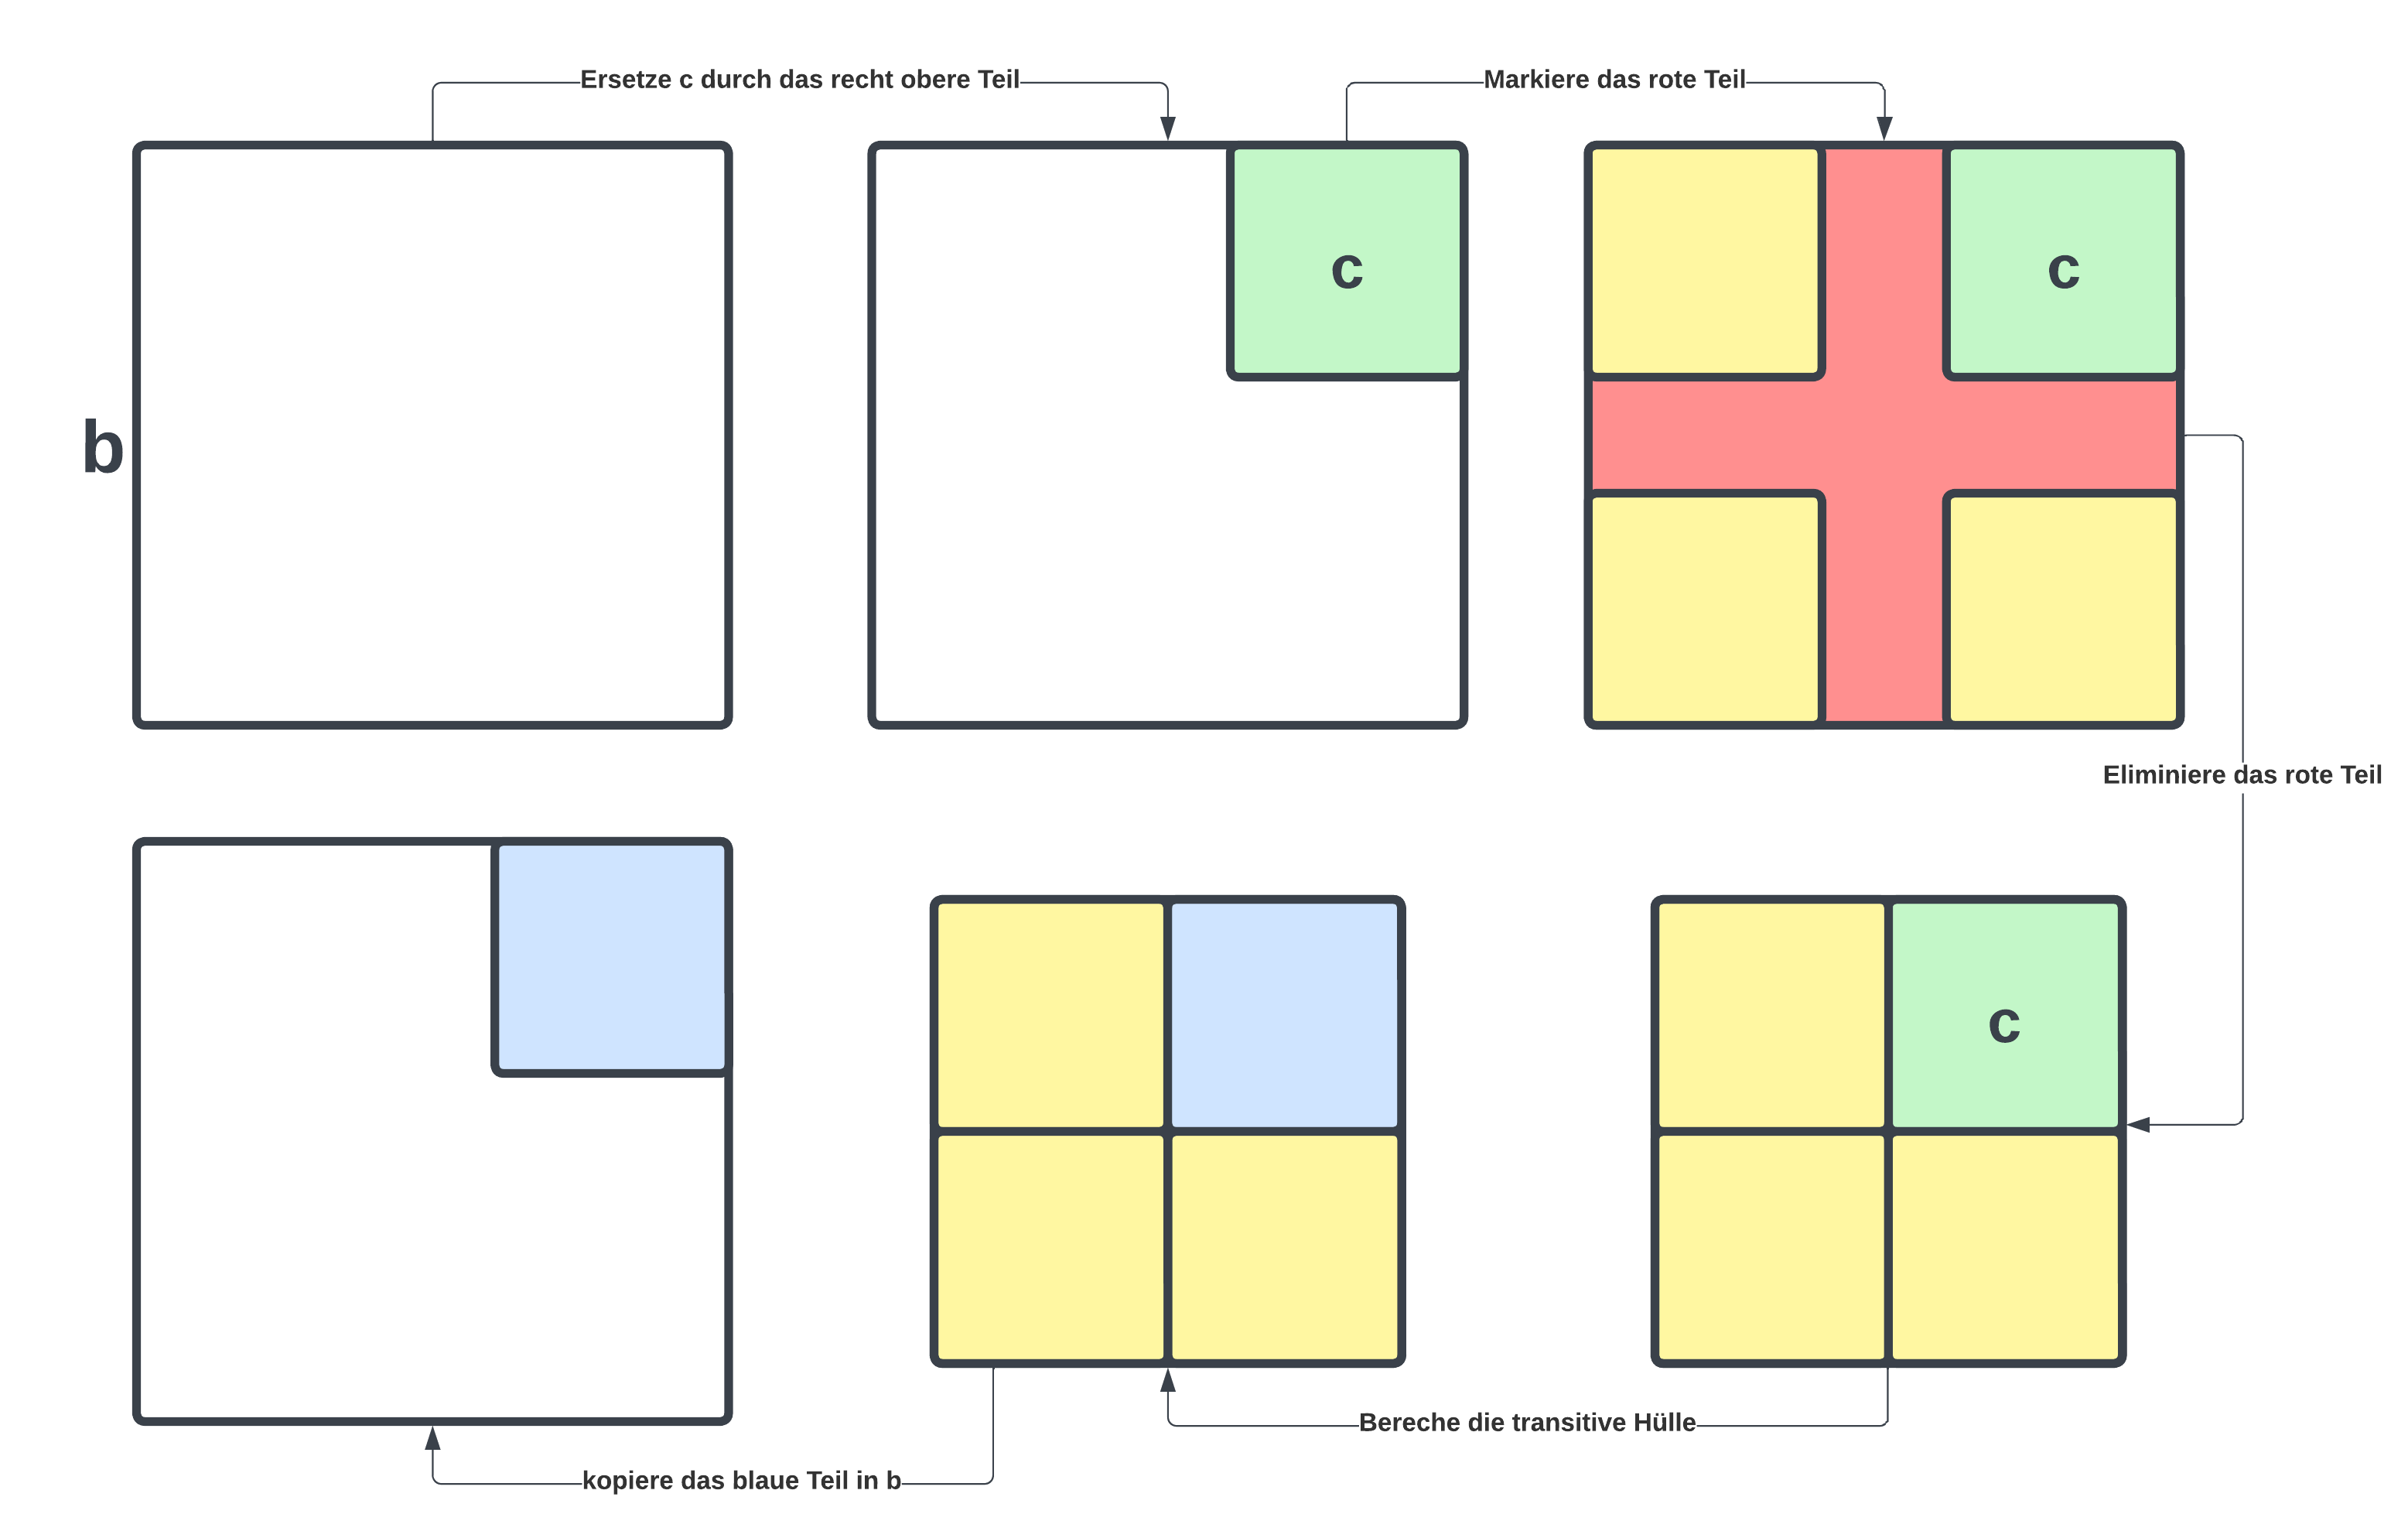
\includegraphics[width=10.5cm,height=7.5cm]{img/LGV10}
%		\end{figure}
%	\end{frame}

	\begin{frame}{Transitive Hülle $\le$ Multiplikation}
		\begin{itemize}
			\item Ersetze die recht obere Partition von $b$ durch $c$. 
		\end{itemize} 
		\begin{figure}
			\centering
			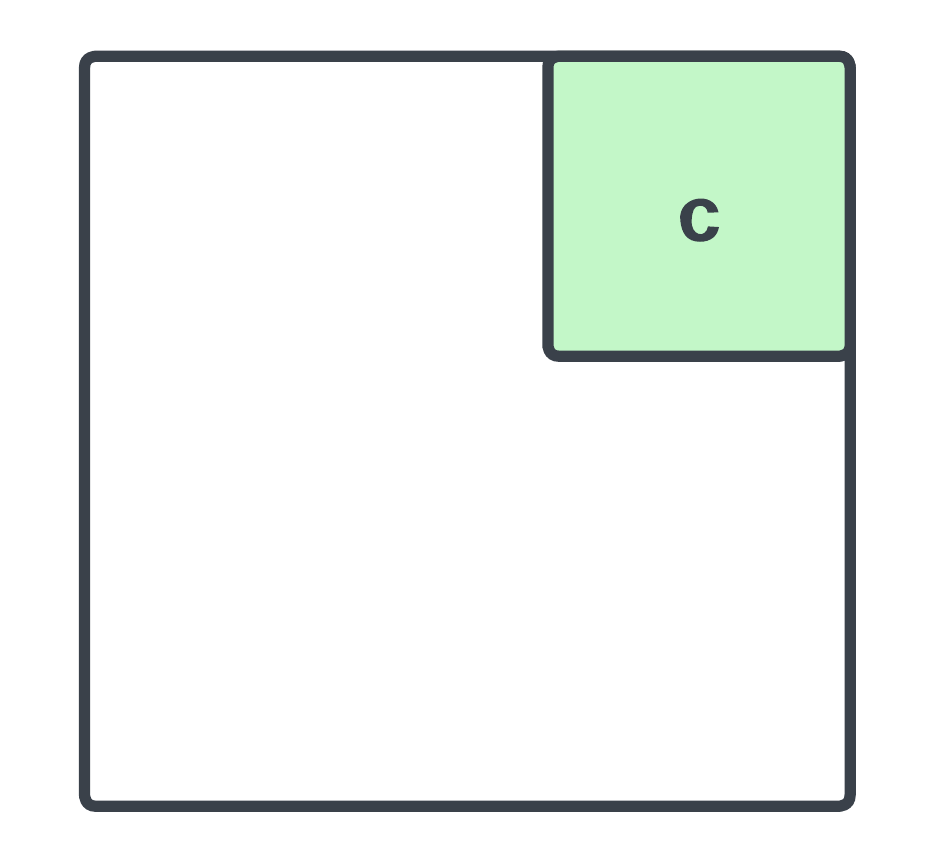
\includegraphics[width=5cm,height=5cm]{img/LGV5}
		\end{figure}
	\end{frame}

	\begin{frame}{Transitive Hülle $\le$ Multiplikation}
		\begin{itemize}
			\item Markiere alle $i$-ten Zeilen und $i$-ten Spalten für $n-r < i \le r$ in rot. 
		\end{itemize} 		
		\begin{figure}
			\centering
			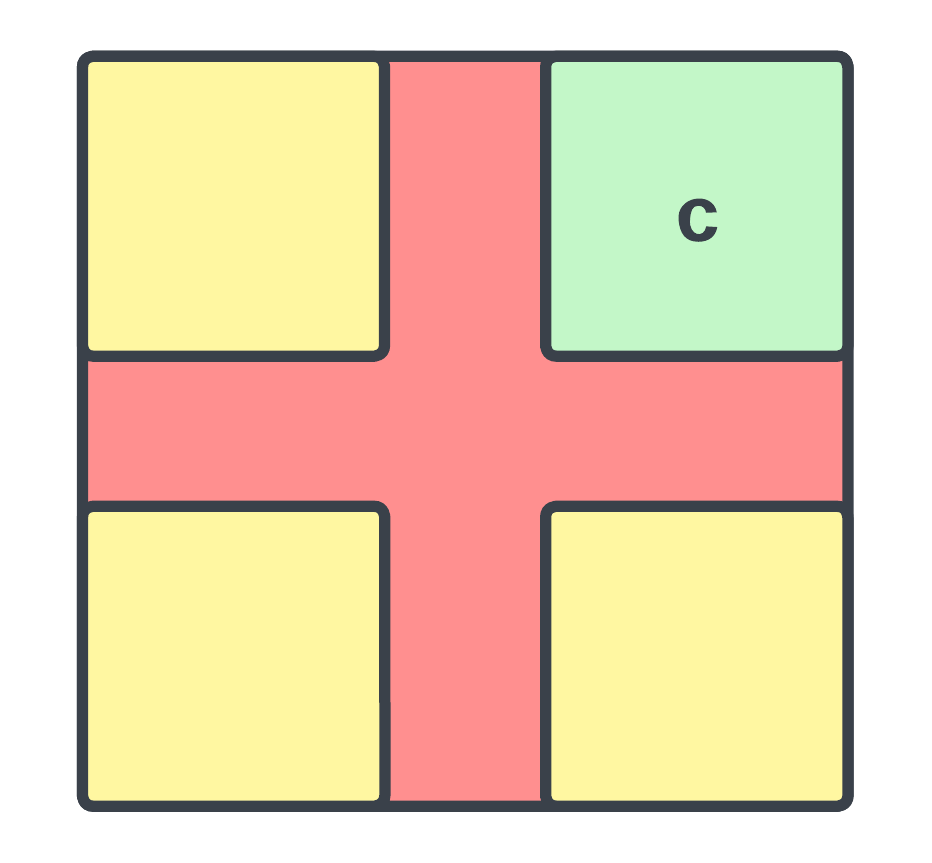
\includegraphics[width=5cm,height=5cm]{img/LGV6}
		\end{figure}
	\end{frame}

	\begin{frame}{Transitive Hülle $\le$ Multiplikation}
		\begin{itemize}
			\item Eliminiere die rot markierten Zeilen und Spalten. 
		\end{itemize} 
		\begin{figure}
			\centering
			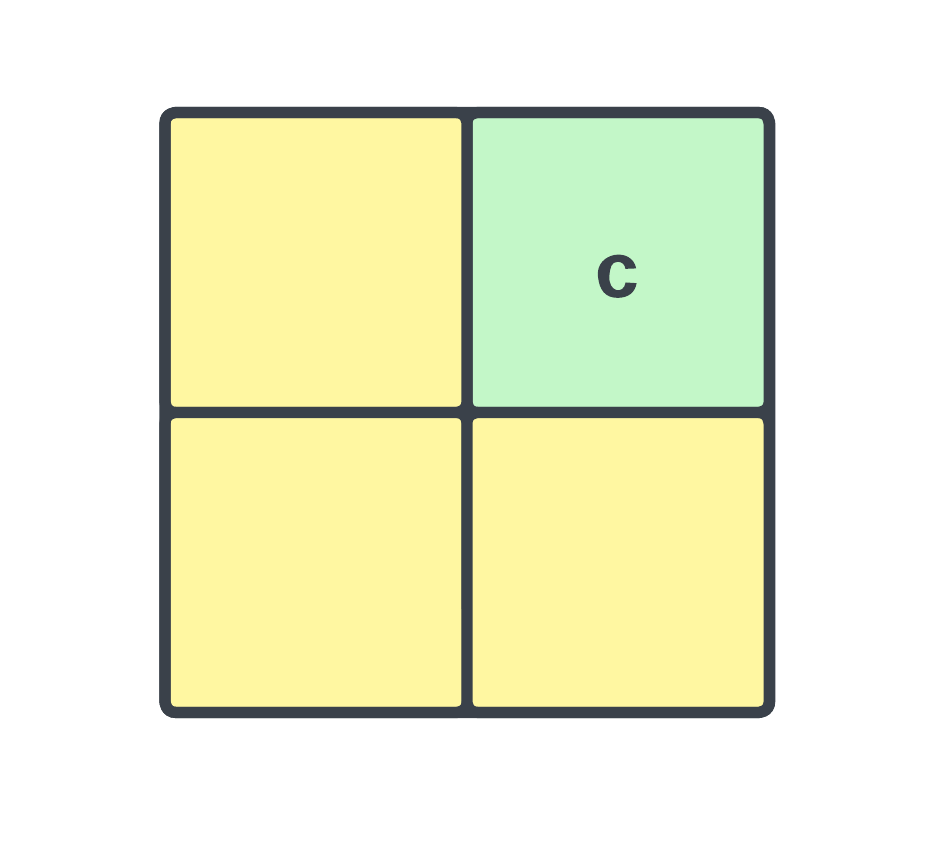
\includegraphics[width=7cm,height=7cm]{img/LGV7}
		\end{figure}
	\end{frame}

	\begin{frame}{Transitive Hülle $\le$ Multiplikation}
		\begin{itemize}
			\item Berechne die transitive Hülle.
		\end{itemize} 
		\begin{figure}
			\centering
			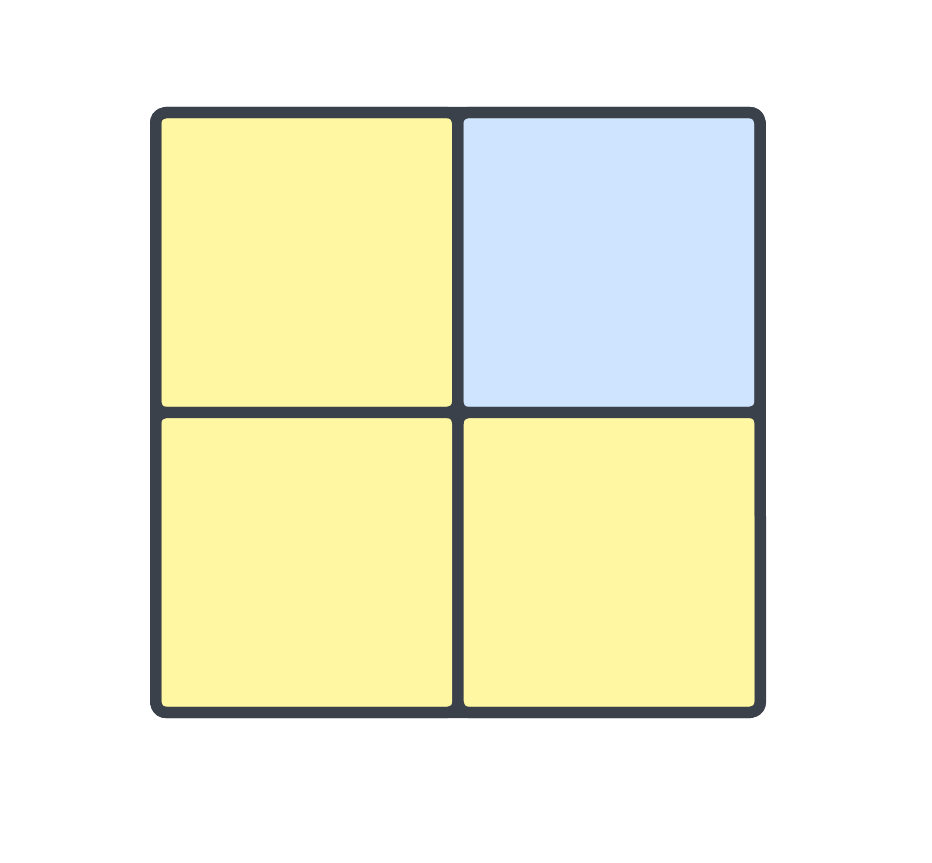
\includegraphics[width=7cm,height=7cm]{img/LGV8}
		\end{figure}
	\end{frame}

	\begin{frame}{Transitive Hülle $\le$ Multiplikation}
		\begin{itemize}
			\item Ersetze die recht obere Partition von $b$ durch die blau markierte Partition. 
		\end{itemize} 
		\begin{figure}
			\centering
			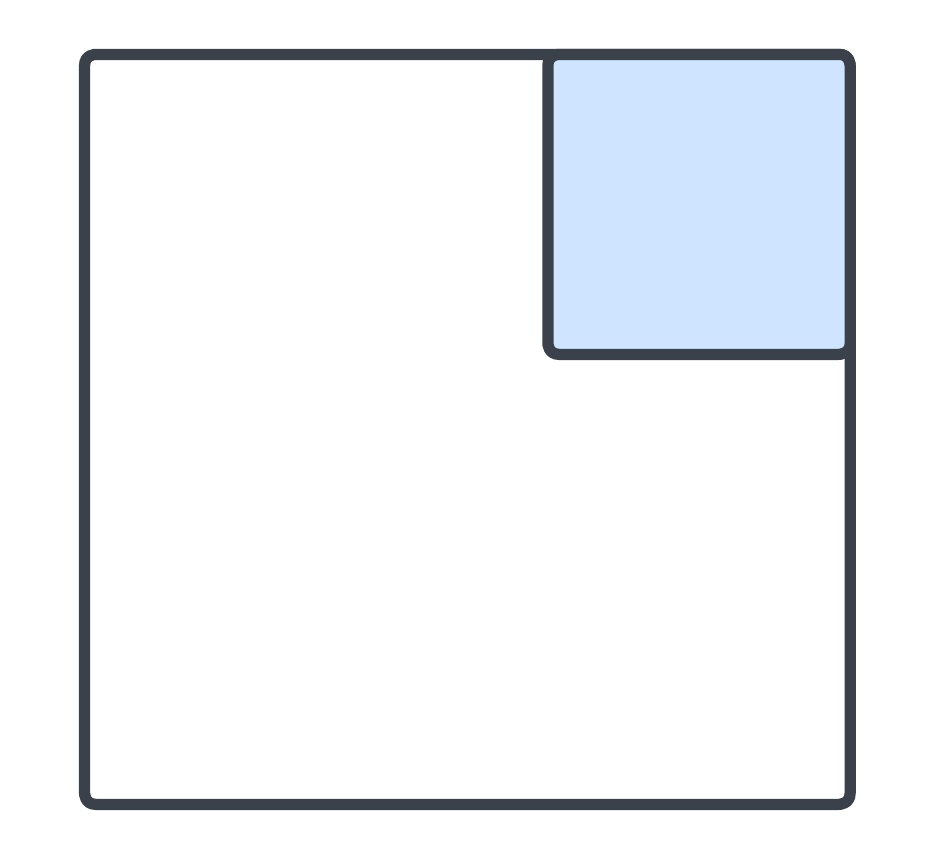
\includegraphics[width=7cm,height=7cm]{img/LGV9}
		\end{figure}
	\end{frame}

%	\begin{frame}{Transitive Hülle $\le$ Multiplikation}
%			\begin{algorithm}[H]
%			\addtocounter{algorithm}{-1}
%			\caption{Lemma Teil 2}
%			\begin{algorithmic}[1]
%				\algrestore{t}
%				\State $d = b$
%				\State Ersetze den oberen rechten Teil von $d$ durch $c$.
%				\State $d[1 \le i \le n-r; r < j \le n] = c$
%				\State Eliminiere alle $i$-ten Zeilen und $i$-ten Spalten für $n-r < i \le r$.
%				\State $d_{partition_1} = d[1 \le i \le n-r; 1 < j \le n-r]$
%				\State $d_{partition_2} = d[1 \le i \le n-r; r < j \le n]$
%				\State $d_{partition_3} = d[r \le i \le n; 1 < j \le n-r]$
%				\State $d_{partition_4} = d[r \le i \le n; r < j \le n]$
%				\State $d = 	
%				\begin{bmatrix}
%					d_{partition_1} & d_{partition_2}\\
%					d_{partition_3} & d_{partition_4}
%				\end{bmatrix}$
%				\State Berechne die transitive Hülle von $d$.
%				\State $theorem2(d)$
%				\State Kopiere den oberen rechten Teil von $d$ in $b$.
%				\State $b[1 \le i \le n-r; r < j \le n] = d[1 \le i \le n-r; n-r < j \le 2*(n-r)]$
%			\end{algorithmic}
%		\end{algorithm} 
%	\end{frame}

	\begin{frame}{Transitive Hülle $\le$ Multiplikation}
		\begin{block} {Theorem}
			\begin{itemize}
				\item $M(n)$ ist die Zeitkomplexität eines Matrixmultiplikationsalgorithmus
				$$T(n) \le M(n) \cdot f(n)$$
				\item wobei $f(n)$ eine konstante Funktion ist, falls für einige $\gamma  > 2$ gilt. Außerdem ist in jedem Fall $f(n) = O(\log n)$. 
			\end{itemize}
		\end{block}
		\pause
		Beweis. 
		\begin{itemize}
			\item Sei $b$ eine $n \times n$ obere Dreieckmatrix
			\item $P_k$ ist die Operation, die ihre Hülle finden soll, wenn jene ihrer folgenden Partitionen bereits bekannt sind
			\begin{itemize}
				\item $[1 \le i, j \le n - \dfrac{n}{k}]$
				\item $[\dfrac{n}{k} < i, j \le n]$
			\end{itemize}
		\end{itemize}
	\end{frame}

	\begin{frame}{Transitive Hülle $\le$ Multiplikation}
		Forts. Beweis.
		\begin{itemize}
			\item Für $k = 2,\ 3$ und $4$ kann rekursiv wie folgt definiert werden:
			\item $P_2: \quad$
			\begin{itemize}
				\item (i) Anwendung von $P_2$ auf die Partition $[\dfrac{n}{4} < i, j\le \dfrac{3n}{4}]$
				\item (ii) Anwendung von $P_3$ auf die Partition $[1 \le i, j\le \dfrac{3n}{4}]$.
				\item (ii) Anwendung von $P_3$ auf die Partition $[\dfrac{n}{4} < i, j\le n]$.
				\item (iii) Anwendung von $P4$.
			\end{itemize}
			\pause
			\item $P_3:\quad$ Anwendung von dem Verfahren des Lemmas für $r = \dfrac{2n}{3}$.
			\pause
			\item $P_4: \quad$ Anwendung von dem Verfahren des Lemmas für $r = \dfrac{3n}{4}$.
		\end{itemize}
	\end{frame}

	\begin{frame}{Transitive Hülle $\le$ Multiplikation}
		\begin{figure}
			\centering
			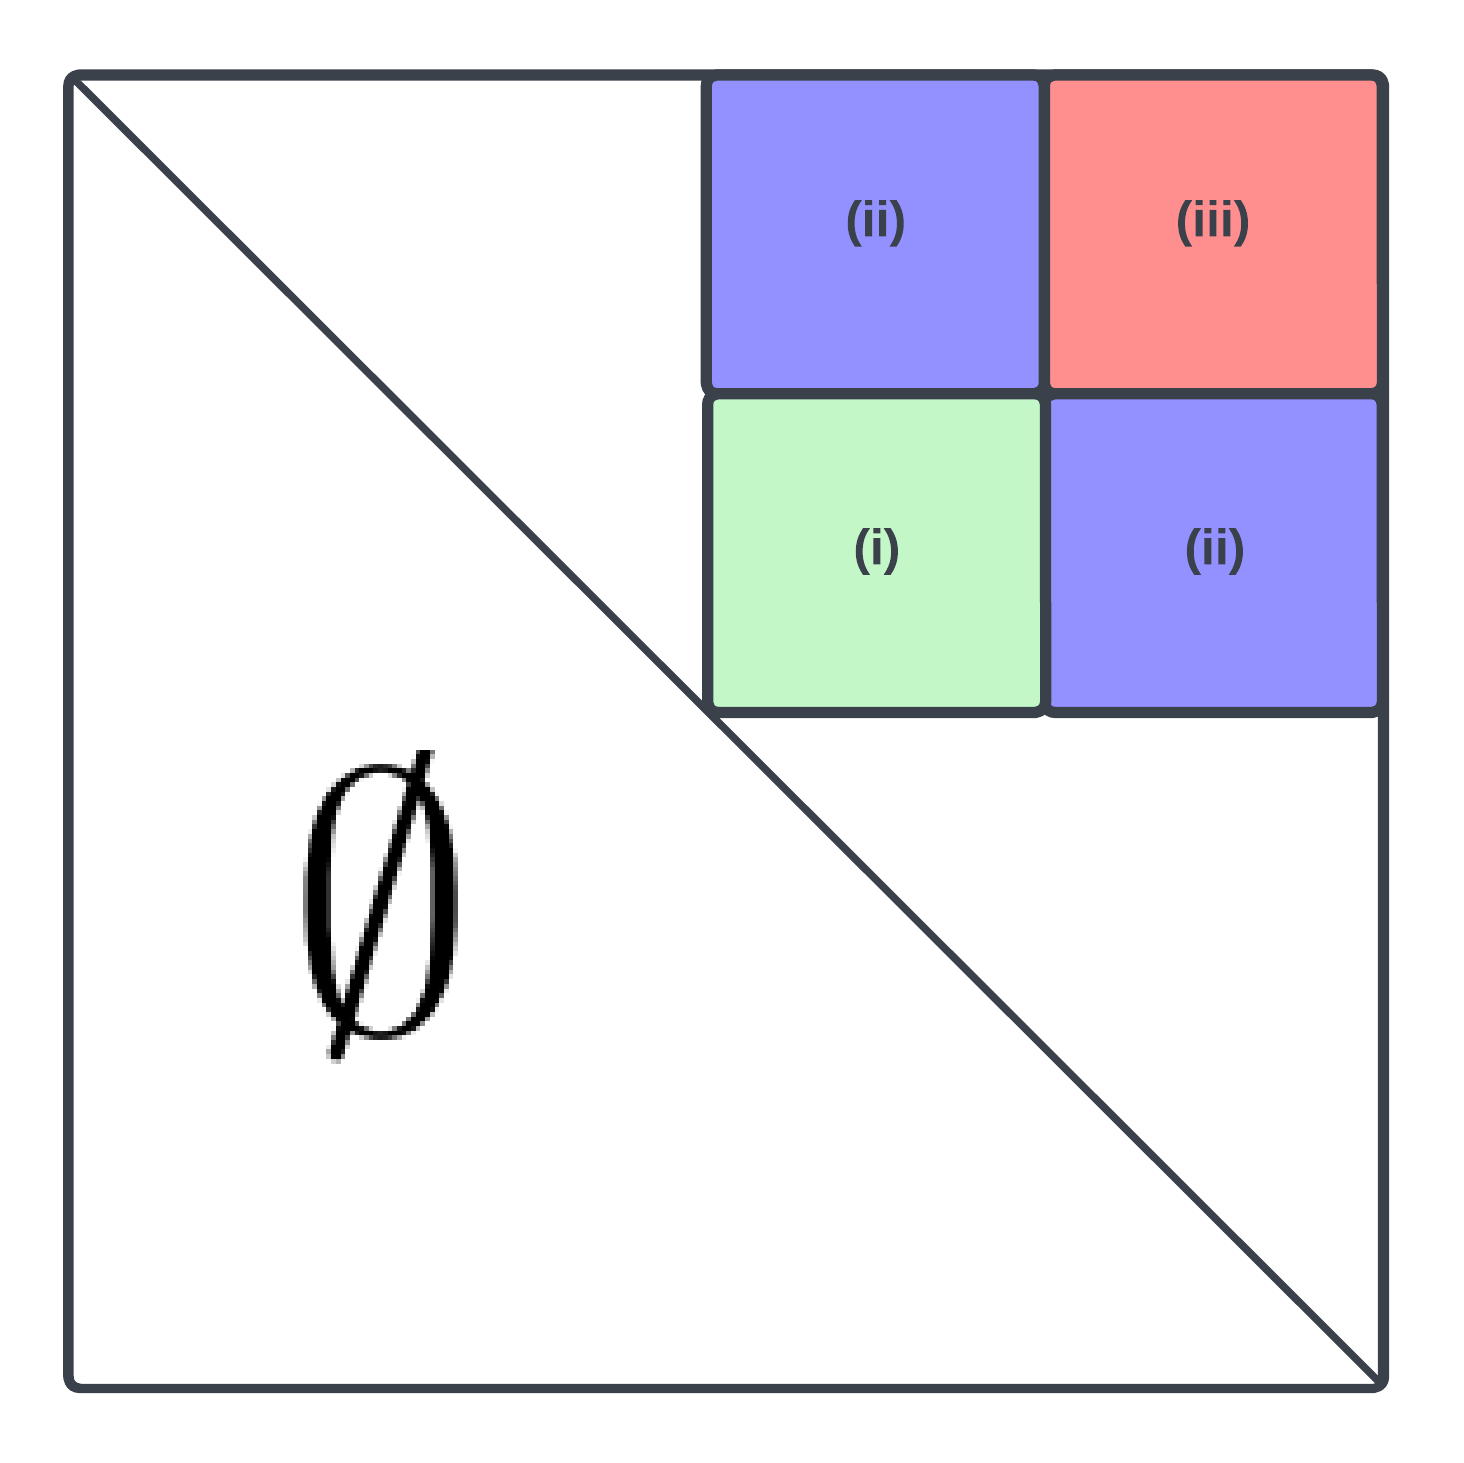
\includegraphics[width=7cm,height=7cm]{img/LGV11}
		\end{figure}
	\end{frame}

	\begin{frame}{Transitive Hülle $\le$ Multiplikation}
		\begin{figure}
			\centering
			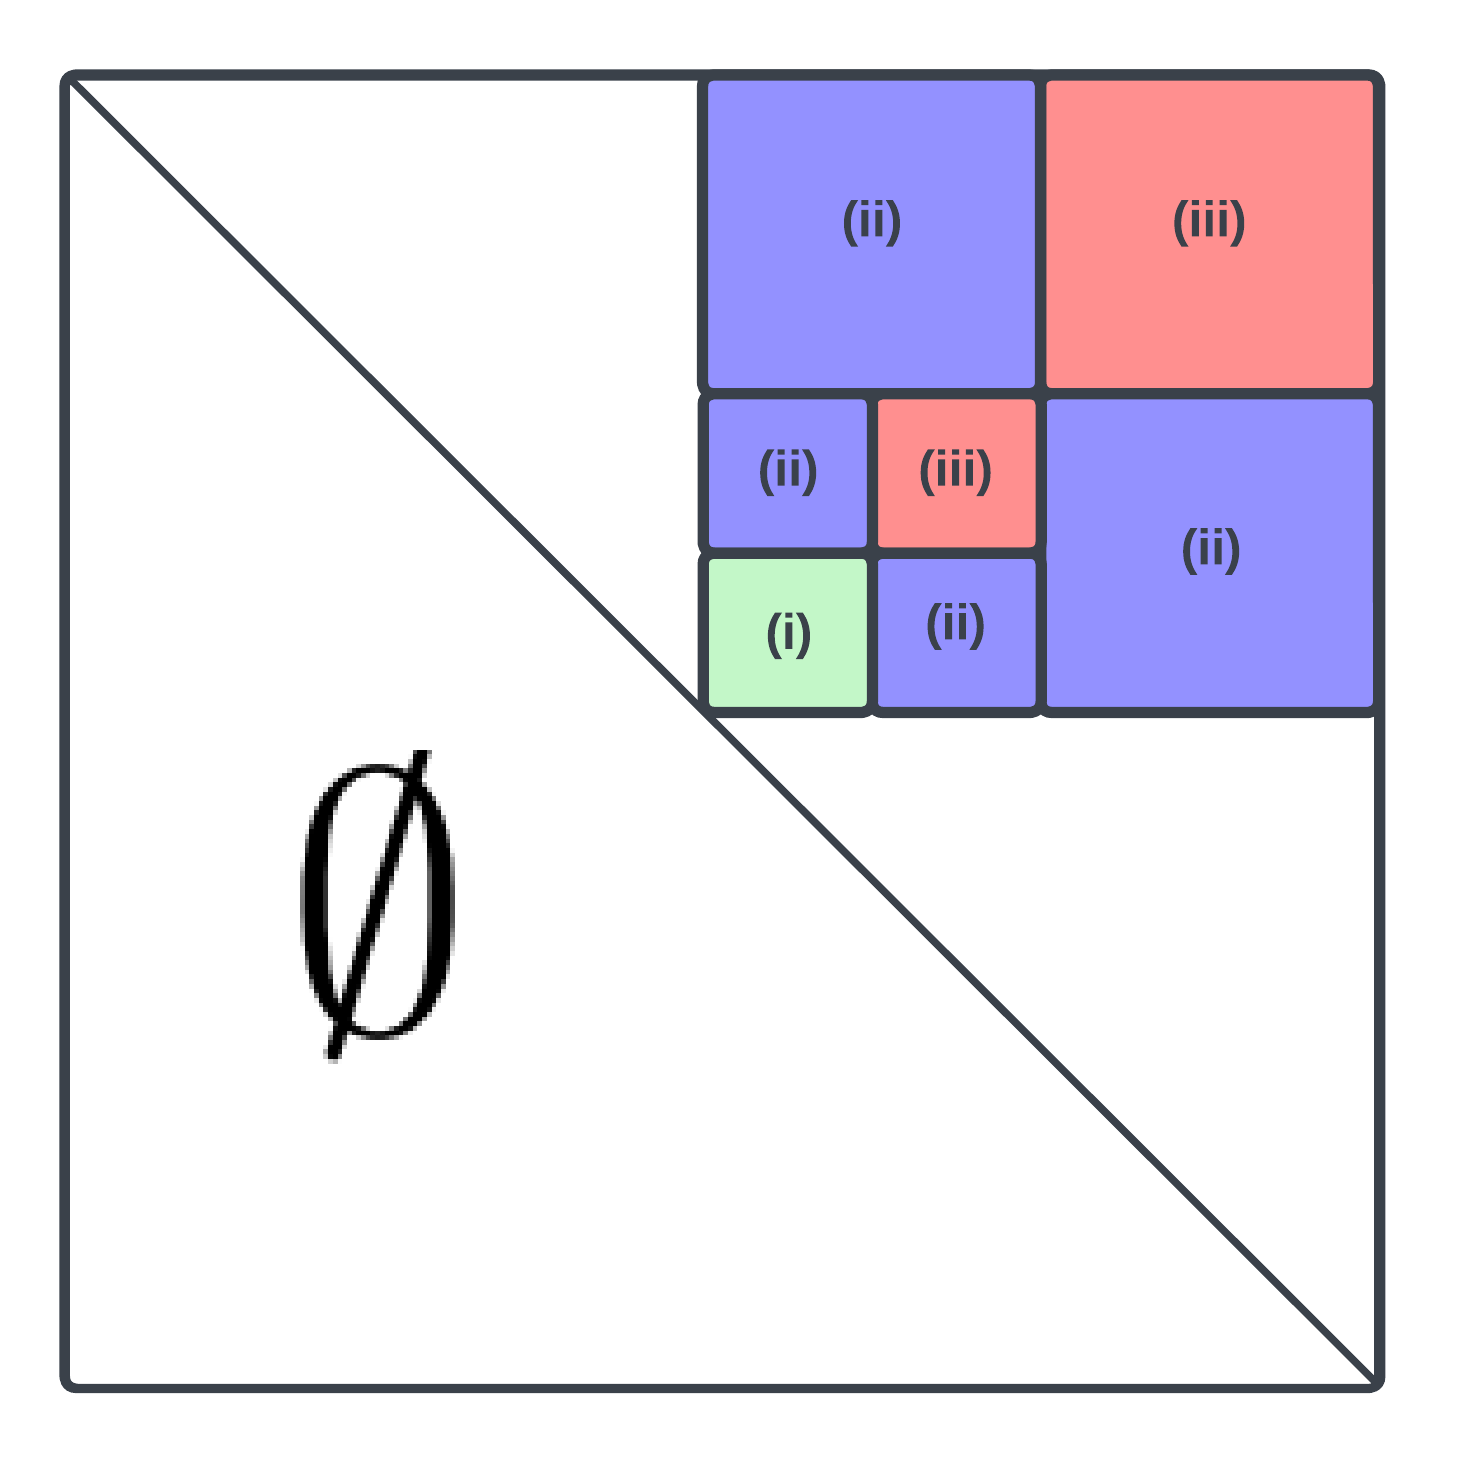
\includegraphics[width=7cm,height=7cm]{img/LGV12}
		\end{figure}
	\end{frame}

	\begin{frame}{Transitive Hülle $\le$ Multiplikation}
		\begin{figure}
			\centering
			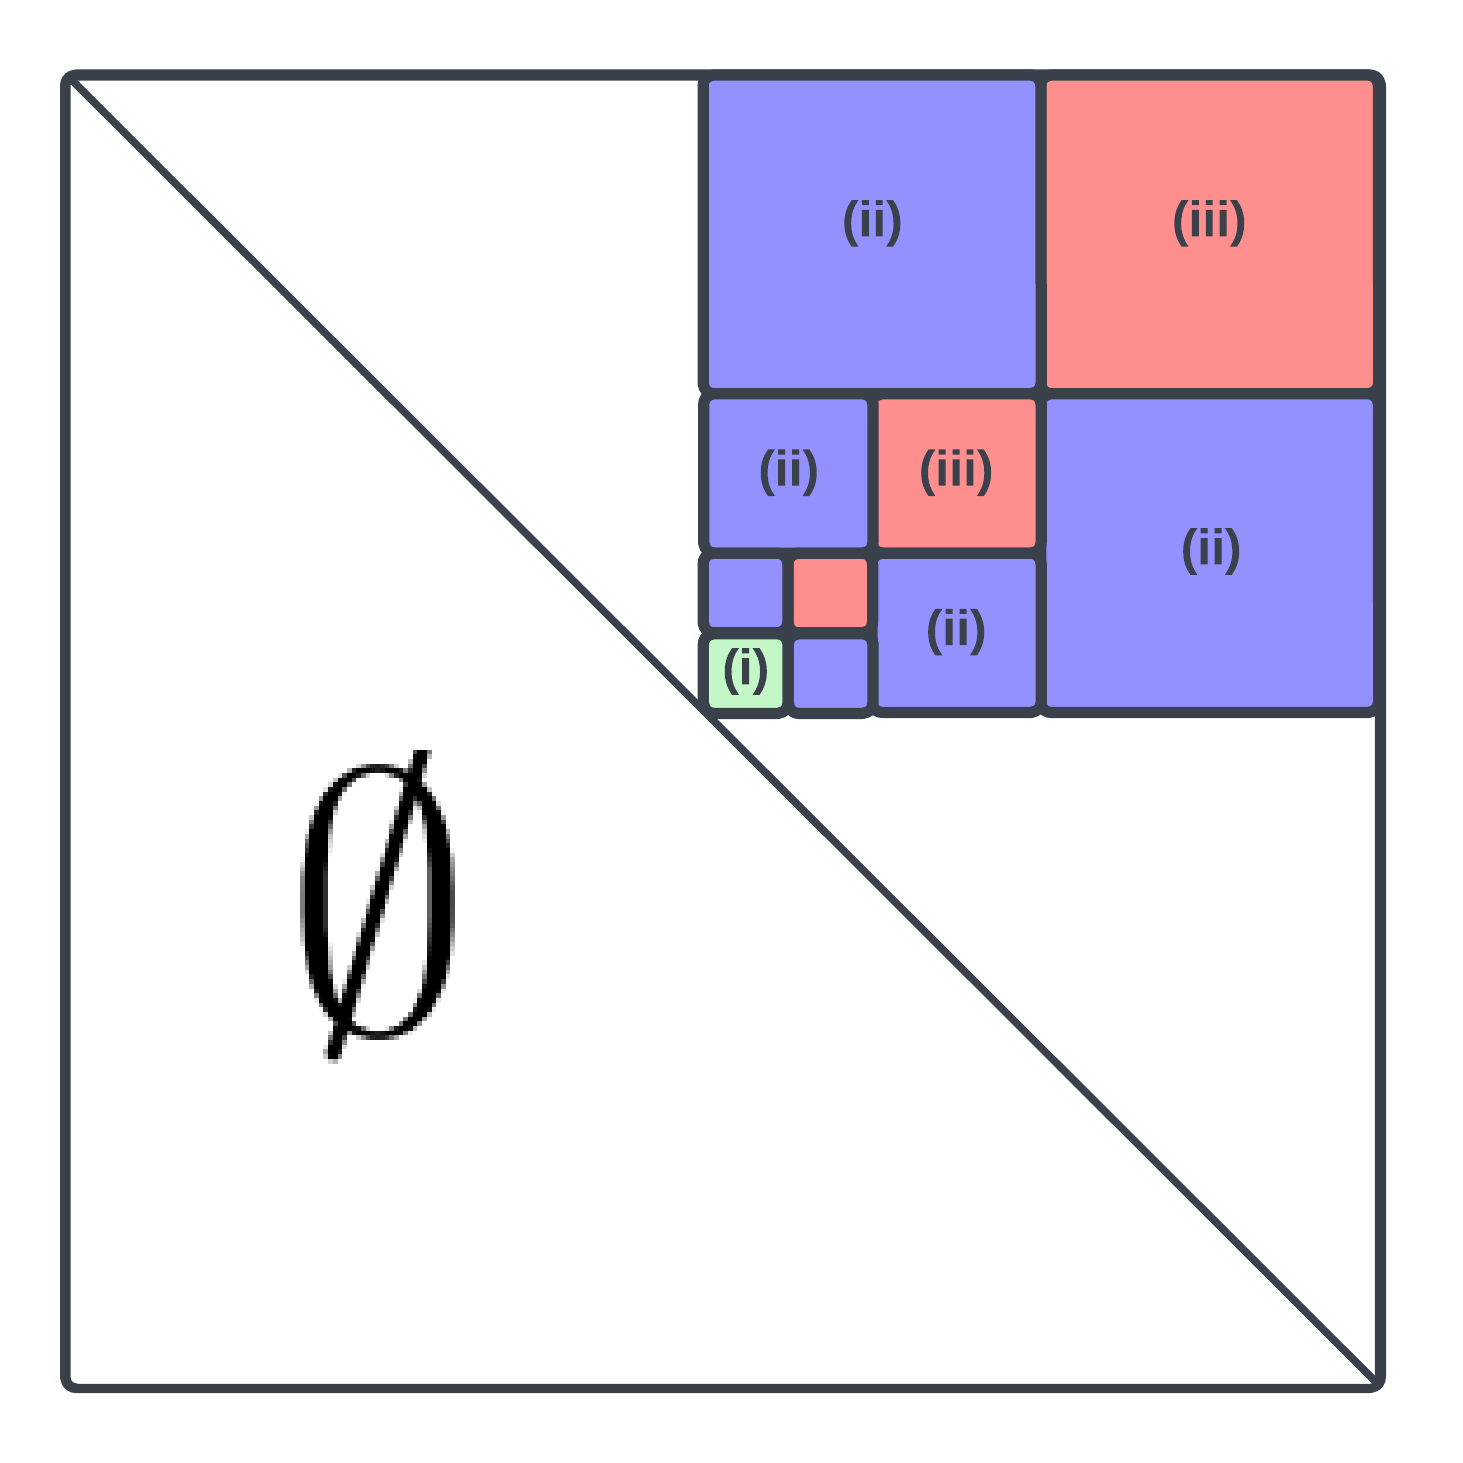
\includegraphics[width=7cm,height=7cm]{img/LGV13}
		\end{figure}
	\end{frame}

	\begin{frame}{Transitive Hülle $\le$ Multiplikation}
		\begin{itemize}
			\item $T_i(n)$ die Zeitschranke der Prozedur $P_i$
			$$
			\begin{aligned}
				& T_2(n) \leq T_2(\dfrac{n}{2})+2 T_3(\dfrac{3n}{4})+T_4(n), \\
				& T_3(n) \leq M(n)+T_2(\dfrac{2n}{3})+O\left(n^2\right), \\
				& T_4(n) \leq M(n)+T_2(\dfrac{n}{2})+O\left(n^2\right). \\
				& \text{Setze } T_3 \text{ und } T_4 \text{ in } T_2 \text{ ein }\\
				& T_2(n) \leq 4 T_2(n / 2)+3 M(n)+O\left(n^2\right)
			\end{aligned}
			$$
			\pause
			\item Unter der Annahme, dass $n$ eine Potenz von 2 ist und
			 \item $\gamma \geq 2$ ist Wachstumsfaktor derart, dass für alle m $M\left(2^{\mathrm{m}+1}\right) \geq 2^\gamma M\left(2^{\mathrm{m}}\right)$
			$$
			T_2(n) \leq O\left(n^2 \log n\right)+3 M(n) \cdot \sum_{m=0}^{\log n}2^{(2-\gamma) m}
			$$
		\end{itemize}
	\end{frame}

	\begin{frame}{Transitive Hülle $\le$ Multiplikation}
		\begin{itemize}
			\item Aber $\sum_{m=0}^{\infty }{x^m}$ konvergiert, wenn $|x| < 1$. Wenn also $\gamma  > 2$,
			$$
			T_2(n) \leq M(n) \cdot \text { Konstante }
			$$
			\item 	Wenn $\gamma = 2$, dann
			$$T_2(n) \le M(n) \cdot \log n \cdot \text { Konstante}$$
			\pause
			\item Der Abschluss von $b$, wobei deren Partitionen $[1 \le i,j\le \dfrac{n}{2}]$ und $[\dfrac{n}{2} < i, j\le n]$ abgeschlossen sind.
			$$T(n) = 2T(\dfrac{n}{2}) + T_2(n) + O\left(n^2\right).$$
			$$
			T(n) \leq O\left(n^2\right)+T_2(n) \cdot \sum_{m=0}^{\log n}2^{-m} \leq 2T_2(n) + O\left(n^2\right).
			$$
		\end{itemize}
	\end{frame}

	\begin{frame}{Multiplikation $\le$ Boolesche Multiplikation}
		\begin{block}{Theorem}
			$M(n) \le BM(n) \cdot Konstante$
		\end{block}
		Beweis. 
		\begin{itemize}
			\item Sei $G = (S, \Sigma, N, P)$ eine Grammatik in Chomsky-Normalform und seien $a$ und $b$ zwei $n \times n$ Matrizen mit $a_{ij},b_{ij}\subseteq N$ für $i,j\in\{1,\ldots ,n\}$
			$$c = a\cdot b$$
			\pause
			\item $2|N|$ booleschen Matrizen $a[N_i], b[N_i]$ für $i=1,\ldots,|N|$ mit $N_i$ bzw. $i$-ten nichtterminalen Zeichen 
			$$a[N_i]_{jk} = 1 \ falls \ N_i \in a_{jk}, \ \ \ \ \ b[N_i]_{jk} = 1 \ falls \ N_i \in b_{jk}$$
		\end{itemize}
	\end{frame}

	\begin{frame}{Multiplikation $\le$ Boolesche Multiplikation}
		Forts. Beweis. 
		\begin{itemize}
			\pause
			\item Für jedes Paar $N_i,\ N_j$ wird dann die boolesche Matrix $c[N_i, N_j]$ für $i.j \in \{1,\ldots,|N|\}$ berechnet, wobei
			$$c[N_i,\ N_j] = a[N_i] \times b[N_j]$$
			\pause
			\item Dies erfordert ${|N|}^2$ boolesche Matrixmultiplikationen. Offensichtlich kann $c$ dann direkt erhalten werden, da nach der Konstruktion $N_k \in c_{ij} \ falls$
			$$\exists N_i,\ N_j \ so dass, \ c[N_i,\ N_j] = 1 \ and\ N_k \to N_i N_j  \in P$$
		\end{itemize}
	\end{frame}
	

	%---------------------------------------------------------
	
	
	
	
	\section{Boolesche-Strassen-Matrix-Multiplikation}

	\begin{frame}{Strassen}
		\begin{block}{Matrix-Multiplikation}
			$$
			\begin{bmatrix}
				a_{11} & a_{12}\\
				a_{21} & a_{22} 
			\end{bmatrix}
			\times
			\begin{bmatrix}
				b_{11} & b_{12}\\
				b_{21} & b_{22}
			\end{bmatrix}
			=
			\begin{bmatrix}
				a_{11} b_{11}  + a_{12} b_{21} & a_{11} b_{12} + a_{12} b_{22}\\
				a_{21} b_{11} + a_{22} b_{21} & a_{21} b_{12} + a_{22} b_{22}
			\end{bmatrix}
			$$
		\end{block}
		\pause
		\begin{block}{Strassen-Matrix-Multiplikation}
			$$
			\begin{bmatrix}
				a_{11} & a_{12}\\
				a_{21} & a_{22} 
			\end{bmatrix}
			\times
			\begin{bmatrix}
				b_{11} & b_{12}\\
				b_{21} & b_{22}
			\end{bmatrix}
			=
			\begin{bmatrix}
				M_{1} + M_{2} - M_{4} + M_{6} & M_{4} + M_{5}\\
				M_{6} + M_{7} & M_{2} - M_{3} + M_{5} - M_{7}
			\end{bmatrix}
			$$	
		\end{block}
		\pause
		\begin{itemize}
			\item $M_{1} = (a_{12} - a_{22}) \cdot (b_{21} + b_{22})$ 
			\item $M_{2} = (a_{11} + a_{22}) \cdot (b_{11} + b_{22})$
			\item $M_{3} = (a_{11} - a_{21}) \cdot (b_{11} + b_{12})$
			\item $M_{4} = (a_{11} + a_{12}) \cdot b_{22}$
			\item $M_{5} = a_{11} \cdot (b_{12} - b_{22})$
			\item $M_{6} = a_{22} \cdot (b_{21} - b_{11})$
			\item $M_{7} = (a_{21} + a_{22}) \cdot b_{11}$
		\end{itemize}
	\end{frame}

	\begin{frame}{Implementierung Strassen}
		\begin{algorithm}[H]
			{Algorithmus}
			\setstretch{1.1}
			\caption[Strassen-Matrix-Multiplikation]{Strassen-Matrix-Multiplikation}
			\begin{algorithmic}[1]
				\Require $(A, \ B)$
				\Ensure $A \times B$
				\If{$length(A) = 1, 2, 4, 8, 16, n^2$}  \ \ \ \ \ \ \ \ \ \ \ \ \ \ \ \ \ \ \ \ \ \ \ \ \ \ \ \ \ \ \ \ \ \ \textbf{\{Basisfall\}}
				\State $A \times B$
				\Else  \ \ \ \ \ \ \ \ \ \ \ \ \ \ \ \ \ \ \ \ \ \ \ \ \ \ \ \ \ \ \ \ \ \ \ \ \ \ \ \ \ \ \ \ \ \ \ \ \ \ \ \ \ \ \ \ \ \ \ \textbf{\{rekursiver Fall\}}
				\State $$
				\begin{bmatrix}
					A_{11} \vline A_{12}\\ \hline
					A_{21} \vline A_{22} 
				\end{bmatrix}
				\
				\begin{bmatrix}
					B_{11} \vline B_{12}\\ \hline
					B_{21} \vline B_{22}
				\end{bmatrix}
				$$
				
				\algstore{t}
			\end{algorithmic}
		\end{algorithm} 
	\end{frame}

	\begin{frame}{Implementierung Strassen}
		\begin{algorithm}[H]
			\begin{algorithmic}[1]
				\algrestore{t}
				\State $m_1$ = Strassen-Matrix-Multiplikation($(a_{12} - a_{22}) ,\ (b_{21} + b_{22})$)
				\State $m_2$ = Strassen-Matrix-Multiplikation($(a_{11} + a_{22}) ,\ (b_{11} + b_{22})$)
				\State $m_3$ = Strassen-Matrix-Multiplikation($(a_{11} - a_{21}) ,\ (b_{11} + b_{12})$)
				\State $m_4$ = Strassen-Matrix-Multiplikation($(a_{11} + a_{12}) ,\ b_{22}$)
				\State $m_5$ = Strassen-Matrix-Multiplikation($a_{11} ,\ (b_{12} - b_{22})$)
				\State $m_6$ = Strassen-Matrix-Multiplikation($a_{22} ,\ (b_{21} - b_{11})$)
				\State $m_7$ = Strassen-Matrix-Multiplikation($(a_{21} + a_{22}) ,\ b_{11}$)
				\State $c_{11} = m_{1} + m_{2} - m_{4} + m_{6}$
				\State $c_{12} = m_{4} + m_{5}$
				\State $c_{21} = m_{6} + m_{7}$
				\State $c_{22} = m_{2} - m_{3} + m_{5} - m_{7}$
				\State return 
				$\begin{bmatrix}
					C_{11} & C_{12}\\
					C_{21} & C_{22}
				\end{bmatrix}$
				\EndIf
			\end{algorithmic}
		\end{algorithm} 
	\end{frame}
		 
	\begin{frame}{Zeitkomplexität Strassen}
		\begin{itemize}
			\item Sei $T_M(n)$ bzw. $T_A(n)$ die Anzahl der Multiplikationen und Additionen.
			\pause
			\item Für $T_M(n)$ gilt:
			$$
			T_M(n) = 
			\begin{cases}
				1, & n=1\\
				7 \cdot T_M(n \textfractionsolidus 2), & n>1 
			\end{cases}
			$$
			\pause
			\item Daraus ergibt sich:
			$$T_M(n) = \underbrace{7 \cdot 7 \ldots 7}_{(\log n)-mal} = 7^{\log n} = n^{\log 7} \le n^{2.8074}$$
			\pause
			\item Für $T_A(n)$ gilt:
				$$
			T_A(n) = 
			\begin{cases}
				0, & n=1\\a
				18(n\textfractionsolidus 2) (n\textfractionsolidus 2) + 7T_A(n\textfractionsolidus 2), & n>1 
			\end{cases}
			$$
			\pause
			\item Damit erhalten wir $T_A(n) = O(n^{2.8074})$.
		\end{itemize}
	\end{frame}

	\begin{frame}{Boolesche Strassen}
		\begin{itemize}
			\item Für die normale Matrix-Multiplikation könnte die boolesche Variante wie folgt aussehen:
			\[
			c_{ij} = \bigvee_{k=1}^n a_{ik} \land b_{kj}
			\]
			\pause
			\item Jedoch ist diese Formel nicht ausreichend für Strassen, da in dessen Berechnung auch Subtraktion involviert ist.
			\pause
			\item Die boolesche Matrix-Multiplikation kann durch die Integer-Matrix-Multiplikation simuliert werden. Wenn die Multiplikation abgeschlossen ist, werden die $0$-Einträge der Matrix $C$ durch $0$ und alle anderen Einträge durch $1$ ersetzt.
		\end{itemize}
	\end{frame}
	
	\begin{frame}{Zeitkomplexität Boolesche Strassen}
		\begin{algorithm}[H]
			\floatname{algorithm}{Algorithmus}
			\setstretch{1.1}
			\caption[Boolean-Strassen]{Boolean-Strassen}
			\label{algorithm20}
			\begin{algorithmic}[1]
				\Require $(A, \ B)$
				\Ensure $A \times B$
				\State $c$ = Strassen-Matrix-Multiplikation-Algorithmus$(A ,\ B$) \textbf{$ \%O(n^{2.8074})$}
				\State $c \ ist \ eine \ n \times m \ Matrix$
				\For{\texttt{$i:=1 \ to \ n$}} \ \ \ \ \ \ \ \ \ \ \ \ \ \ \ \ \ \ \ \ \ \ \ \ \ \ \ \ \ \ \ \ \ \ \ \ \ \textbf{$ \%O(n)$ Durchläufe}
				\For{\texttt{$j:=1 \ to \ m$}} \ \ \ \ \ \ \ \ \ \ \ \ \ \ \ \ \ \ \ \ \ \ \ \ \ \ \ \ \ \ \ \textbf{$ \%O(m)$ Durchläufe}
				\If{$c[i][j] \neq 0$}
				\State $c[i][j] = 1$
				\EndIf
				\EndFor
				\EndFor
				\State return $c$
			\end{algorithmic}
		\end{algorithm}
	\end{frame}

%	\begin{frame}[plain]
%		\begin{table}[H]
%			\centering
%			\begin{tabular}{|m{2cm}||m{2.5cm}|m{2.5cm}|m{2.5cm}|} 
%				\hline
%				\diagbox[width=\dimexpr \textwidth/8+3\tabcolsep\relax, height=1cm]{}{}& $1000\times 1000$ & $2000\times2000$ & $4000\times4000$ \\ [0.5ex] 
%				\hline\hline
%				$n=1$ & $3918.410s$ & $27363.411s$ & $100\ldots00 s$\\[1ex]
%				\hline
%				$n=2$ & $774.119s$ & $5483.681s$ & $100\ldots00 s$\\[1ex]
%				\hline
%				$n=4$ & $117.295s$ & $823.133s$ & $5770.478s$\\[1ex]
%				\hline
%				$n=8$ & $21.732s$ & $145.509s$ & $967.924s$\\[1ex]
%				\hline
%				$n=16$ & $6.765s$ & $36.112s$ & $216.553s$\\[1ex]
%				\hline
%				$n=32$ & $3.905s$ & $19.076s$ & $93.765s$\\[1ex]
%				\hline
%				$n=64$ & $3.606s$ & $14.754s$ & $68.552s$\\[1ex]
%				\hline
%				$n=128$ & $3.466s$ &$14.826s$ &$63.704s$\\[1ex]
%				\hline
%				$n=256$ & $3.167s$ & $13.505s$ &$58.498s$\\[1ex]
%				\hline
%				$n=512$ & $3.244s$ & $12.964s$ & $54.527s$\\[1ex]
%				\hline
%				$n=1024$ & $3.891s$ & $12.716s$ & $52.362s$\\[1ex]
%				\hline
%				$n=2048$ & $3.817s$ & $34.466s$ & $51.265s$\\[1ex]
%				\hline
%			\end{tabular}
%		\end{table}
%	\end{frame}

	\section{Zeitergebnisse}
	
	\begin{frame}{CYK-Algorithmus vs. LGV-Algorithmus}
		1. Test: Grammatiken mit einem nichtterminalen Zeichen und unterschiedlicher Anzahl von Produktionen
		\pause
		\begin{itemize}
			\item $G_1 = (S, \{a\}, \{S\}, \{S\to SS | a\})$
			\item $G_2 = (S, \{a,b,c,d\}, \{S\}, \{S\to SS | a | b | c |d\})$
		\end{itemize}
		\pause
		\begin{table}[H]
			\centering
			\begin{tabular}{|m{2cm}||m{1.7cm}|m{1.7cm}||m{1.7cm}|m{1.7cm}|} 
				\hline
				\multirow{2}{*}{\diagbox[width=\dimexpr \textwidth/8+4.5\tabcolsep\relax, height=1cm]{$|w|$}{$Grammatik$}}& \multicolumn{2}{c||}{$|N|=1 \ |P|=2$} & \multicolumn{2}{c|}{$|N|=1 \ |P|=5$}\\ [0.5ex] 
				\cline{2-5}
				& CYK & LGV & CYK & LGV\\
				\hline\hline
				$254$ & $9.429s$ & $14.008s$ &$10.658s$&$13.820s$\\[1ex]
				\hline
				$510$ & $82.134s$ & \cellcolor{lightgray}$81.0641s$ & $90.295s$&\cellcolor{lightgray}$79.939s$\\[1ex]
				\hline
				$1022$ & $649.915s$ & \cellcolor{green}$457.080s$ & $717.655s$&\cellcolor{green}$454.532s$\\[1ex]
				\hline
				$2046$ & $5192.263s$ & $2571.086s$ & $5740.248s$&$2585.514s$\\[1ex]
				\hline
				$4094$ & $41030.947s$ & $14531.633s$ & $48343.457s$&$14539.953s$\\[1ex]
				\hline
				$8190$ & $\ldots s$ & $\ldots s$ & $\ldots s$ & $\ldots s$ \\[1ex]
				\hline
			\end{tabular}
		\end{table}
	\end{frame}

	
	%---------------------------------------------------------
	
	\begin{frame}{CYK-Algorithmus vs. LGV-Algorithmus}
		2. Test: Grammatiken mit unterschiedlicher Anzahl von nichtterminalen Zeichen
		\pause
		\begin{itemize}
			\item $G_3 = (S, \{a,b\}, \{S,B\}, \{S\to SB | BS | a | b ,B\to b\})$
			\item $G_4 = (S, \{a,b\}, \{S,A,B\}, \{S\to SB | SA | a | b ,B\to b\ ,A\to a\})$
		\end{itemize}
		\pause
		\begin{table}[H]
			\centering
			\begin{tabular}{|m{2cm}||m{1.7cm}|m{1.7cm}||m{1.7cm}|m{1.7cm}|}  
				\hline
				\multirow{2}{*}{\diagbox[width=\dimexpr \textwidth/8+4.5\tabcolsep\relax, height=1cm]{$|w|$}{$Grammatik$}}& \multicolumn{2}{c||}{$|N|=2$}  & \multicolumn{2}{c|}{$|N|=3$}\\ [0.5ex] 
				\cline{2-5}
				& CYK & LGV & CYK & LGV \\
				\hline\hline
				$254$ & $10.382s$& $23.382s$&$12.145s$& $35.979s$\\[1ex]
				\hline
				$510$ & $86.694s$& $134.923s$& $97.738s$& $207.755s$\\[1ex]
				\hline
				$1022$ & $730.844s$& \cellcolor{lightgray}$771.789s$& $804.681s$& $1180.179s$\\[1ex]
				\hline
				$2046$ & $5706.038s$& \cellcolor{green}$4365.122s$&$6311.629s$& \cellcolor{lightgray}$6685.876s$\\[1ex]
				\hline
				$4094$ & $46464.972s$& $24703.334s$& $51015.653s$& \cellcolor{green}$37991.584s$\\[1ex]
				\hline
				$8190$ & $\ldots s$& $\ldots s$& $\ldots s$& $\ldots s$\\[1ex]
				\hline
			\end{tabular}
		\end{table}
	\end{frame}
	
	%---------------------------------------------------------
	
	\begin{frame}{CYK-Algorithmus vs. LGV-Algorithmus}
		3. Test: Grammatik mit vier nichtterminalen Zeichen
		\pause
		\begin{itemize}
			\item $G_5 = (S, \{a,b\}, \{S,A,B,C\},$ \\ $ \{S\to AB | AC ,C\to SB,B\to b\ ,A\to a\})$
		\end{itemize}
		\pause
		\begin{table}[H]
			\centering
			\begin{tabular}{|m{2.5cm}||m{2cm}|m{2cm}|} 
				\hline
				\multirow{2}{*}{\diagbox[width=\dimexpr \textwidth/8+5.3\tabcolsep\relax, height=1.1cm]{$|w|$}{$Grammatik$}}& \multicolumn{2}{c|}{$|N|=4$}\\ [0.5ex] 
				\cline{2-3}
				& CYK & LGV \\
				\hline\hline
				$254$ & $12.120s$& $53.519s$\\[1ex]
				\hline
				$510$ & $99.725s$& $305.683s$\\[1ex]
				\hline
				$1022$ & $824.670s$& $1744.574s$\\[1ex]
				\hline
				$2046$ & $6353.308s$& $9999.785s$\\[1ex]
				\hline
				$4094$ & $51319.035s$& \cellcolor{lightgray}$55878.540s$\\[1ex]
				\hline
				$8190$ & $\ldots s$& \cellcolor{green}$\ldots s$\\[1ex]
				\hline
			\end{tabular}
		\end{table}
	\end{frame}
	
	%---------------------------------------------------------
	
	\begin{frame}{Einfluss der Nichtterminalen auf den LGV-Algorithmus}
		\begin{itemize}
			\item LGV-Algorithmus Verhältnis bzgl. $|N|$ für ein Wort der Länge $|w| = 4094$
		\end{itemize}
		\begin{figure}[H]
			\begin{tikzpicture}[scale=0.9]
				\begin{axis}[
					%		title={nothing},
					xlabel={Anzahl der nichtterminalen Zeichen $|N|$},
					ylabel={Zeit in Stunden},
					%			ymin=0, ymax=130,
					%			xmin=0, xmax=146,
					xtick={1,2,3,4,5},
					%			ytick={0,1,2,4,8,16,32,64,128,256},
					ymajorgrids=true,
					grid style=dashed,
					]
					
					\addplot[
					color=blue,
					mark=otimes*,
					]
					coordinates {
						(1,4.038)(2,6.862)(3,10.553)(4,15.521)
					};
					
					%			\legend{$CYK$,$LGV$}
				\end{axis}
			\end{tikzpicture}
		\end{figure}
	\end{frame}

	\begin{frame}{Einfluss der Nichtterminalen auf den LGV-Algorithmus}
		\begin{block}{Fundamentalsatz der Zeitergebnisse}
			Für jede Grammatik mit $|N|$ nichtterminalen Zeichen ein Wort der Länge $|w| = n$ existiert, wo der LGV-Algorithmus den CYK-Algorithmus ab diesem Wort zeitlich besiegt.
		\end{block}
	\end{frame}
	
	%---------------------------------------------------------
	
%	\begin{frame}{Wichtige Fragestellungen}
%		\begin{itemize}
%			\item Warum wurden die Wortlängen $|w| = 2^n-2$ für $n = 8,9,10,11,12$ und $13$ so gewählt?
%			\pause
%			\item Welche Sprachen erzeugen die Grammatiken $G_1, G_2, G_3, G_4$ und $G_5$? Sind diese Sprachen rein kontextfrei?
%		\end{itemize}
%		\pause
%		\begin{figure}[H]
%			\begin{tikzpicture}[scale=5]
%				\node[above,ellipse,minimum height=4em,minimum width=4em,draw] (a) {Typ 3: Reguläre Sprachen};
%				\node[above,ellipse,minimum height=7em,minimum width=20em,draw] (b) {};
%				\node[above,ellipse,minimum height=10em,minimum width=25em,draw] (c) {};
%				\node[above,ellipse,minimum height=13em,minimum width=30em,draw] (d) {};
%				\path (a.north) node[above] {Typ 2: Kontextfreie Sprachen}
%				(b.north) node[above] {Typ 1: Kontextsensitive Sprachen}
%				(c.north) node[above] {Typ 0: Aufzählbare Sprachen};
%			\end{tikzpicture}
%			\label{Chomsky-Hierarchie}
%		\end{figure}
%	\end{frame}

	%---------------------------------------------------------
	
	\section{Zusammenfassung}

	\begin{frame}{Zusammenfassung}
		Wortproblem für kontextfreie Sprachen in subkubischer Zeit:
		\pause
		\begin{itemize}
			\item Umwandlung der kontextfreien Grammatiken in Chomsky-Normalform
			\pause
			\item Der CYK-Algorithmus hat eine Zeitkomplexität von $O(n^{3})$
			\pause
			\item Der LGV-Algorithmus hat eine Zeitkomplexität von $O(n^{2.81})$
			\pause
			\item Durchgeführte Tests zwischen den beiden Algorithmen auf dem Uni-Cluster
			\pause
			\begin{itemize}
				\item Verwendung großer Wörter mit Längen zwischen $254$ und $8190$
				\item Auswahl von Grammatiken mit unterschiedlicher Anzahl an nichtterminalen Zeichen
			\end{itemize}
			\pause
			\item Schlussfolgerung der Tests: Fundamentalsatz
		\end{itemize}
	\end{frame}
	%---------------------------------------------------------

%	\section{Refernces}
%	\begin{frame}
%		\frametitle{References}
%		\begin{thebibliography}{999}
%			
%			\bibitem[1]{simon-theorem}
%			Imre Simon. Factorization forests of finite height. \emph{Theoretical Computer
%				Science}, 72(1):65–94, 1990.
%			
%			\bibitem[2]{theorem-original}
%			Mikołaj Bojańczyk. Factorization Forests. \emph{Developments in Language Theory}, 2009.
%			
%		\end{thebibliography}
%	\end{frame}



\end{document}